% Defining schemes
\begin{topic}{ringed-space}{(locally) ringed space}
    A \textbf{ringed space} is a pair $(X, \mathcal{O}_X)$ consisting of a \tref{TO:topological-space}{topological space} $X$ and a \tref{sheaf}{sheaf} of rings $\mathcal{O}_X$ on $X$.
    
    A morphism of ringed spaces from $(X, \mathcal{O}_X)$ to $(Y, \mathcal{O}_Y)$ is a pair $(f, f^\#)$ of a continuous map $f : X \to Y$ and a map $f^\# : \mathcal{O}_Y \to f_* \mathcal{O}_X$ of sheaves of rings on $Y$.
    
    A ringed space $(X, \mathcal{O}_X)$ is a \textbf{locally ringed space} if for each point $x \in X$, the \tref{stalk}{stalk} $\mathcal{O}_{X,x}$ is a \tref{AA:local-ring}{local ring}.
    
    A morphism of locally ringed spaces is a morphism $(f, f^\#)$ of ringed spaces such that for each point $x \in X$ the induced map of local rings $f^\#_x : \mathcal{O}_{Y, f(x)} \to \mathcal{O}_{X, x}$ is a \textit{local morphism}, i.e. the pre-image of the maximal ideal of $\mathcal{O}_{X, x}$ is the maximal ideal of $\mathcal{O}_{Y, f(x)}$.
\end{topic}

\begin{topic}{spectrum-ring}{spectrum of a ring}
    Let $R$ be a \tref{AA:ring}{commutative ring}. The \textbf{spectrum} of $R$ is the \tref{ringed-space}{locally ringed space} $(X, \mathcal{O}_X)$ defined as follows.
    \begin{itemize}
        \item The topological space $X$ is the set of \tref{AA:prime-ideal}{prime ideals} of $R$, whose closed sets are given precisely by the sets $V(I) = \{ \textup{prime ideals } \mathfrak{p} \textup{ with } \mathfrak{p} \supset I \}$ for all ideals $I$ of $R$.
        \item The \tref{sheaf}{sheaf} of rings $\mathcal{O}_X$ is given as follows. For each open set $U \subset X$, $\mathcal{O}_X(U)$ is the set of functions $s : U \to \sqcup_{\mathfrak{p} \in U} R_\mathfrak{p}$ with $s(\mathfrak{p}) \in R_\mathfrak{p}$ for each $\mathfrak{p} \in U$, such that $s$ is locally a quotient of elements of $R$. This means that for each $\mathfrak{p} \in U$, there is a neighborhood $V \subset U$ of $\mathfrak{p}$, and elements $a, f \in R$ such that for each $\mathfrak{q} \in V$, $f \not\in \mathfrak{q}$ and $s(\mathfrak{q}) = a/f$ in $A_\mathfrak{q}$. The sets $\mathcal{O}_X(U)$ are indeed rings.
    \end{itemize}
    The spectrum of $R$ is denoted $\Spec R$.
\end{topic}

\begin{example}{spectrum-ring}
    While $\mathcal{O}_X(D_f) = R_f$ is a localization for \tref{principal-open-subset}{principal opens} $D_f = \{ \mathfrak{p} \in \Spec R \mid f \not\in \mathfrak{p} \}$, generally for open $U$ the ring $\mathcal{O}_X(U)$ need not be a localization of $R$.
    
    Namely, let $k$ be a field and consider $R = k[x, y, z, w] / (xy - zw)$, and let $U = D_y \cup D_z$. The elements $w/y \in R_y = \mathcal{O}_X(D_y)$ and $x/z \in R_z = \mathcal{O}_X(D_z)$ are equal in the localization $R_{yz} = \mathcal{O}_X(D_{yz})$, so they glue to an element $f \in \mathcal{O}_X(U)$. However, if $f = g/h$ for some $g, h \in R$, then we must have $h \in (y, z)$, but then $h$ vanishes somewhere on $U$.
\end{example}

\begin{topic}{scheme}{scheme}
    A \textbf{scheme} is a \tref{ringed-space}{locally ringed space} $(X, \mathcal{O}_X)$ in which every point has an open neighborhood $U$ such that $(U, \mathcal{O}_X|_U)$ is isomorphic to the \tref{spectrum-ring}{spectrum} of a \tref{AA:ring}{ring}. A morphism of schemes is a morphism of locally ringed spaces.
    
    One calls $X$ the \textit{underlying topological space}, and $\mathcal{O}_X$ its \textit{structure sheaf}.
\end{topic}

\begin{topic}{affine-scheme}{affine scheme}
    A \tref{scheme}{scheme} is \textbf{affine} if it is isomorphic to the \tref{spectrum-ring}{spectrum} of a \tref{AA:ring}{ring}.
\end{topic}

\begin{topic}{principal-open-subset}{principal open subset}
    A \textbf{principal open subset} of an \tref{affine-scheme}{affine scheme} $\Spec R$ is an open subset of the form
    \[ (\Spec R)_f = \{ \mathfrak{p} \in \Spec R : f \not\in \mathfrak{p} \} \]
    for some $f \in R$.
\end{topic}

% Scheme properties
\begin{topic}{reduced-scheme}{reduced scheme}
    A \tref{scheme}{scheme} $X$ is \textbf{reduced} if for every open subset $U \subset X$ the ring $\mathcal{O}_X(U)$ is \tref{AA:reduced-ring}{reduced}.
    
    Equivalently, this is the case if all stalks $\mathcal{O}_{X, x}$ are reduced.
\end{topic}

\begin{topic}{integral-scheme}{integral scheme}
    A \tref{scheme}{scheme} $X$ is \textbf{integral} if it is non-empty and for every non-empty open subset $U \subset X$ the ring $\mathcal{O}_X(U)$ is a \tref{AA:domain}{domain}.
    
    Equivalently, this is the case if $X$ is \tref{reduced-scheme}{reduced} and \tref{TO:irreducible-space}{irreducible}.
\end{topic}

\begin{topic}{noetherian-scheme}{(locally) noetherian scheme}
    A \tref{scheme}{scheme} $X$ is \textbf{locally noetherian} if it can be covered by open affine subsets $\Spec A_i$, where each $A_i$ is a \tref{AA:noetherian-ring}{noetherian ring}. It is \textbf{noetherian} if it is locally noetherian and \tref{quasi-compact-scheme}{quasi-compact}.
\end{topic}

\begin{topic}{finite-type}{(locally) of finite type}
    A morphism $f : X \to Y$ of \tref{scheme}{schemes} is \textbf{of finite type at $x \in X$} if there exist affine opens $U = \Spec A \subset X$ containing $x$ and $V = \Spec B \subset Y$ with $f(U) \subset V$ such that $A$ is a \tref{AA:finitely-generated-algebra}{finitely generated} $B$-algebra (via the induced map $B \to A$).
    
    The morphism $f$ is \textbf{locally of finite type} if it is of finite type at each $x \in X$, and it is \textbf{of finite type} if it is locally of finite type and \tref{quasi-compact-morphism}{quasi-compact}.
\end{topic}

\begin{topic}{finite-presentation}{(locally) of finite presentation}
    A morphism $f : X \to Y$ of \tref{scheme}{schemes} is \textbf{of finite presentation at $x \in X$} if there exists affine opens $U = \Spec A \subset X$ containing $x$ and $V = \Spec B \subset Y$ with $f(U) \subset V$ such that $A$ is a \tref{AA:finitely-presented-algebra}{finitely presented} $B$-algebra (via the induced map $B \to A$).
    
    The morphism $f$ is \textbf{locally of finite presentation} if it is of finite presentation at each $x \in X$, and it is \textbf{of finite presentation} if it is locally of finite presentation, \tref{quasi-compact-scheme}{quasi-compact}, and \tref{separated-morphism}{quasi-separated}.
\end{topic}

\begin{topic}{finite-morphism}{finite morphism}
    A morphism $f : X \to Y$ of \tref{scheme}{schemes} is \textbf{finite} if there exists a covering of $Y$ by open affine subsets $V_i = \Spec B_i$, such that for each $i$, $f^{-1}(V_i)$ is affine, equal to $\Spec A_i$, where $A_i$ is a $B_i$-algebra which is a \tref{AA:finitely-generated-module}{finitely generated} $B_i$-module.
\end{topic}

\begin{topic}{quasi-finite-morphism}{quasi-finite morphism}
    A morphism $f : X \to Y$ of \tref{scheme}{schemes} is \textbf{quasi-finite} if it is of \tref{finite-type}{finite type}, and every point $x \in X$ is isolated in its fiber $f^{-1}(f(x))$, i.e. every fiber is a discrete finite set.
\end{topic}

\begin{example}{quasi-finite-morphism}
    Every \tref{finite-morphism}{finite morphism} is quasi-finite, but the converse is not true. Namely, consider the immersion
    \[ i : \Spec \ZZ[\tfrac{1}{2}] \to \Spec \ZZ . \]
    Since $i$ is an open immersion, all fibers either consist of a single point or are empty. Furthermore, $i$ is of finite type as $\ZZ[\tfrac{1}{2}]$ is a finitely generated $\ZZ$-algebra, and $i$ is quasi-compact since the source and target are affine, hence $i$ is quasi-finite. However, $i$ is not finite since $\ZZ[\tfrac{1}{2}]$ is not finitely generated as a $\ZZ$-module.
\end{example}

\begin{topic}{open-immersion}{open immersion}
    An \textbf{open immersion} is a morphism $j : U \to X$ of \tref{scheme}{schemes} which induces an isomorphism of $U$ with an open subscheme of $X$.
\end{topic}

\begin{topic}{closed-immersion}{closed immersion}
    A \textbf{closed immersion} is a morphism $i : Z \to X$ of \tref{scheme}{schemes} such that $i$ induces a \tref{TO:homeomorphism}{homeomorphism} of the underlying space of $Z$ onto a closed subset of that of $X$, and furthermore the induced map $i^\# : \mathcal{O}_X \to i_*\mathcal{O}_Z$ of sheaves on $X$ is surjective.
\end{topic}

\begin{topic}{immersion}{immersion}
    An \textbf{immersion} is a morphism $Y \to X$ of \tref{scheme}{schemes} which factors as $j \circ i$, where $i$ is a \tref{closed-immersion}{closed immersion} and $j$ is an \tref{open-immersion}{open immersion}.
    \[ Y \xrightarrow{i} U \xrightarrow{j} X \]
\end{topic}

\begin{topic}{affine-morphism}{affine morphism}
    A morphism $f : X \to Y$ of \tref{scheme}{schemes} is \textbf{affine} if the inverse image of every affine open in $Y$ is an affine open of $X$. 
\end{topic}

\begin{example}{affine-morphism}
    \begin{itemize}
        \item Any morphism $f : \Spec(R) \to \Spec(S)$ between affine schemes is affine.
        \item The inclusion $\iota : \AA^2_k \setminus \{ (0, 0) \} \to \AA^2_k$ is not affine, since $\AA^2_k \setminus \{ (0, 0) \}$ is not affine.
        \item Let $Y_1 = Y_2 = \AA^2_k$, and let $Y$ be obtained by gluing $Y_1$ and $Y_2$ along $\AA^2_k \setminus \{ (0, 0) \}$. Then the inclusions $j_i : Y_i \to Y$ are not affine, since $j_1^{-1}(Y_2) = j_2^{-1}(Y_1) = \AA^2_k \setminus \{ (0, 0) \}$ is not affine.
    \end{itemize}
\end{example}

\begin{topic}{quasi-compact-morphism}{quasi-compact morphism}
    A morphism $f : X \to Y$ of \tref{scheme}{schemes} is \textbf{quasi-compact} if the inverse image of every \tref{TO:compact-space}{compact} open in $Y$ is compact in $X$.
\end{topic}

\begin{topic}{quasi-compact-scheme}{quasi-compact scheme}
    A \tref{scheme}{scheme} $X$ is \textbf{quasi-compact} if its underlying \tref{TO:topological-space}{topological space} is \tref{TO:compact-space}{compact}.
\end{topic}

\begin{example}{quasi-compact-scheme}
    Any affine scheme $X = \Spec R$ is quasi-compact. Since the standard opens form a basis for the topology on $X$, it suffices to consider an open cover of the form $X = \cup_{f \in S} X_f$ for some subset $S \subset R$. Note that $\{ X_f : f \in S \}$ covers $X$ $\iff$ no prime ideal of $R$ contains $S$ $\iff$ $1$ is contained in the ideal generated by $S$. In case of the latter, $1$ is also contained in the ideal generated by some finite $S' \subset S$, so $X = \cup_{f \in S'} X_f$ as well.
\end{example}

\begin{example}{quasi-compact-scheme}
    Let $X = \Spec k[x_1, x_2, \ldots]$ and let $U = X \setminus \{ (x_1, x_2, \ldots) \}$. Since $X$ is affine, it is quasi-compact. However, $U$ is not quasi-compact as the cover $\{ X_{x_i} : i = 1, 2, \ldots \}$ does not admit a finite subcover. Namely, any finite subset $\{ X_{x_{i_1}}, X_{x_{i_2}}, \ldots, X_{x_{i_n}} \}$ will not cover the prime ideal $(x_{i_1}, x_{i_2}, \ldots, x_{i_n})$.
\end{example}

\begin{topic}{normal-scheme}{normal scheme}
    A \tref{scheme}{scheme} $X$ is \textbf{normal} if all of its local rings $\mathcal{O}_{X,x}$ are \tref{AA:integral-closure}{integrally closed} \tref{AA:domain}{domains}.
    % Every scheme can be `normalized'.
\end{topic}

\begin{example}{normal-scheme}
    The cusp $C = \Spec k[x, y] / (x^3 - y^2)$ is not normal since $k[x, y] / (x^3 - y^2)$ is not integrally closed: the element $t = y/x$ is integral, as $t^2 = x$, but does not lie in $k[x, y] / (x^3 - y^2)$.
    
    Adding this element gives
    \[ \begin{aligned}
        k[x, y, y/x] / (x^3 - y^2) &\isom k[t] \\
        x &\mapsto t^2 \\
        y &\mapsto t^3
    \end{aligned} \]
    which is integrally closed. This is the \textit{normalization} of $C$
    \[ \AA_k^1 \to C, \quad t \mapsto (t^2, t^3) . \]
\end{example}

\begin{example}{normal-scheme}
    Let $k$ be a field with $\operatorname{char}(k) \ne 2$, and consider $X = \Spec k[x, y, z] / (z^2 - xy)$. To show $X$ is a normal scheme, we will prove the ring $R = k[x, y, z] / (z^2 - xy)$ is an integrally closed domain. First of all, $R$ is a domain because $z^2 - xy$ is irreducible in $k[x, y, z]$. Note that $K$, the field of fractions of $R$, is a field extension of $k(x, y)$ of degree $2$. Take any element $f = \alpha + \beta z \in K$, with $\alpha, \beta \in k(x, y)$, and assume $f$ is integral over $R$. If the minimal polynomial of $f$ over $R$ is linear, then $f \in R$ and we are done. Otherwise, note that $f$ satisfies $f^2 - 2 \alpha f + (\alpha - \beta^2 xy) = 0$, so that $X^2 - 2 \alpha X + (\alpha^2 - \beta^2 xy)$ must be the minimal polynomial of $f$ over $R$, and hence the coefficients $-2 \alpha$ and $\alpha^2 - \beta^2 xy$ lie in $R$. Since $2$ is invertible in $R$, it follows that $\alpha \in R$ and $\beta^2 xy \in R$. As $xy$ is squarefree, we must have $\beta \in R$, so $f = \alpha + \beta z \in R$, and we conclude that $R$ is integrally closed.
\end{example}

\begin{topic}{separated-scheme}{(quasi-)separated scheme}
    A \tref{scheme}{scheme} $X$ is \textbf{separated} if the morphism $X \to \Spec \ZZ$ is \tref{separated-morphism}{separated}.
    
    A scheme $X$ is \textbf{quasi-separated} if the morphism $X \to \Spec \ZZ$ is \tref{separated-morphism}{quasi-separated}.
\end{topic}

\begin{topic}{separated-morphism}{(quasi-)separated morphism}
    A morphism $f : X \to Y$ of \tref{scheme}{schemes} is \textbf{quasi-separated} if the diagonal $\Delta_{X/Y} : X \to X \times_Y X$ is quasi-compact, and it is \textbf{separated} if the diagonal $\Delta_{X/Y}$ is a closed immersion.
\end{topic}

\begin{example}{separated-morphism}
    Any morphism of affine schemes is separated. Namely, for any $f : \Spec A \to \Spec B$, the diagonal $\Delta$ corresponds to the ring map $A \otimes_B A \to A : a \otimes a' \mapsto aa'$, which is clearly surjective. In this way $A$ is seen as a quotient of $A \otimes_B A$, so $\Delta$ is a closed immersion.
\end{example}

\begin{example}{separated-morphism}
    Let $X$ be the affine line with two origins, that is, glue two copies of $\AA_k^1$ along $\AA_k^1 \setminus \{ 0 \}$. We claim that $X$ is not separated over $k$. Namely, consider the map $\AA^1_k \to X \times_k X$ obtained from the two different maps $\AA_k^1 \to X$. Then the inverse image of the diagonal is $\AA_k^1 \setminus \{ 0 \}$, which is not closed. Hence, the diagonal is not closed and $\Delta$ is not a closed immersion. However, $X$ can be shown to be quasi-separated over $k$.
\end{example}

\begin{example}{separated-morphism}
    Let $X_1 = X_2 = \Spec k[x_1, x_2, \ldots]$ and let $X = X_1 \cup X_2$ glued along the complement of $\{ (x_1, x_2, \ldots) \}$. Now $\Delta_{X/k}^{-1}(X_1 \times X_2) = \Spec k[x_1, x_2, \ldots] \setminus \{ (x_1, x_2, \ldots) \}$ is not \tref{quasi-compact-scheme}{quasi-compact}, although $X_1 \times X_2$ is. Therefore, $X \to \Spec k$ is not quasi-separated, and in particular not separated.
\end{example}

\begin{topic}{proper-morphism}{proper morphism}
    A morphism $f : X \to Y$ of \tref{scheme}{schemes} is \textbf{proper} if it is \tref{separated-morphism}{separated}, \tref{finite-type}{of finite type} and \tref{TO:universally-closed}{universally closed}.
\end{topic}

\begin{example}{proper-morphism}
    Any \tref{closed-immersion}{closed immersion} $i : Y \to X$ is proper. Indeed, the base change of a closed immersion is again a closed immersion, so $i$ is universally closed. Separatedness can be checked locally on the target: if $X = \Spec R$ then $Y = \Spec R / I$ for some ideal $I \subset R$, so $Y$ is also affine, and any morphism between affine schemes is separated. From this local expression of $X$ and $Y$ it is also clear $i$ is of finite type.
\end{example}

\begin{example}{proper-morphism}
    The morphism $\AA_k^1 \to \Spec k$ is not proper as it is not universally closed. Namely, the projection $\AA^1_k \times \AA^1_k \to \AA^1_k$ sends the closed set $\{ xy - 1 = 0 \}$ to $\AA^1_k \setminus \{ 0 \}$ and thus cannot be a closed mapping. However, the morphism is clearly of finite type, and also separated as the diagonal $\Delta : \AA^1_k \to \AA^1_k \times \AA^1_k$ is closed, it is given by $\{ x - y = 0 \}$.
\end{example}

\begin{example}{proper-morphism}
    Let $X$ be the affine line with double origin, i.e. two copies of $\AA^1$ glued along $\AA^1 \setminus \{ 0 \}$. Then $X \to \AA^1$ is of finite type and universally closed (the latter as $X_R \to \AA^1_R$ is closed for all rings $R$). However, $X \to \AA^1$ is not separated and hence not proper. For this we need to show $\Delta_{X / \AA^1} : X \to X \times_{\AA^1} X$ is not a closed immersion. Consider $\AA^1 \to X \times_{\AA^1} X$ induced from the two maps different maps $\AA^1 \to X$, and note that the inverse image of the diagonal is $\AA^1 \setminus \{ 0 \}$ which is not closed. Hence the diagonal is not closed.
\end{example}

\begin{topic}{projective-morphism}{(quasi-)projective morphism}
    A morphism $f : X \to Y$ of \tref{scheme}{schemes} is
    \begin{itemize}
        \item \textbf{projective} (\textit{in the sense of EGA}) if it factors as
        \[ X \xrightarrow{i} \PP(\mathcal{E}) \xrightarrow{\pi} Y \]
        for some \tref{coherent-sheaf}{quasi-coherent} finite type $\mathcal{O}_Y$-module $\mathcal{E}$, with $i$ a \tref{closed-immersion}{closed immersion} and $\pi$ the projection,
        \item \textbf{bundle-projective} if it factors as
        \[ X \xrightarrow{i} \PP(\mathcal{E}) \xrightarrow{\pi} Y \]
        for some finite locally free $\mathcal{O}_Y$-module $\mathcal{E}$, with $i$ a \tref{closed-immersion}{closed immersion} and $\pi$ the projection,
        \item \textbf{H-projective} (\textit{`H' standing for Hartshorne}) if it factors as
        \[ X \xrightarrow{i} \PP^n_Y \xrightarrow{\pi} Y , \]
        for some integer $n \ge 0$, with $i$ a closed immersion and $\pi$ the projection.
        \item \textbf{locally projective} if there exists an open covering $Y = \bigcup_i U_i$ such that $f^{-1}(U_i) \to U_i$ is projective for each $i$.
    \end{itemize}
    The morphism $f$ is \textbf{quasi-projective} if it factors as
    \[ X \xrightarrow{j} X' \xrightarrow{g} Y , \]
    with $j$ an \tref{open-immersion}{open immersion} and $g$ a projective morphism.
\end{topic}

\begin{example}{projective-morphism}
    There are implications
    \[ \textup{H-projective} \Rightarrow \textup{bundle-projective} \Rightarrow \textup{projective} \Rightarrow \textup{locally projective} \]
    but the converses do not hold.
    \begin{itemize}
        \item Let $k$ be a field. The obvious morphism $\bigsqcup_{n = 1}^{\infty} \PP^n_k \to \bigsqcup_{n = 1}^{\infty} \Spec k$ is bundle-projective but not H-projective.
        \item Let $X$ be the affine line over $k$ with infinitely many origins. The morphism $\bigsqcup_{n = 1}^{\infty} \PP^n_k \to X$ which sends $\PP^n_k$ to the $n$-th origin is projective but not bundle-projective.
        \item There are examples of morphisms which are locally projective but not projective.
    \end{itemize}
\end{example}

\begin{topic}{regular-scheme}{regular scheme}
    A \tref{scheme}{scheme} $X$ is \textbf{regular} if it is \tref{noetherian-scheme}{locally noetherian} and all of its stalks are \tref{AA:regular-ring}{regular local rings}.
\end{topic}

\begin{topic}{variety}{variety}
    A \textbf{variety} is a \tref{reduced-scheme}{reduced} \tref{separated-morphism}{separated} \tref{scheme}{scheme} of \tref{finite-type}{finite type} over a \tref{AA:field}{field} $k$.
\end{topic}

\begin{topic}{complete-variety}{complete variety}
    A \tref{variety}{variety} over $k$ is \textbf{complete} if it is \tref{proper-morphism}{proper} over $k$.
\end{topic}

\begin{topic}{geometrically-regular}{geometrically regular}
    Let $X$ be a \tref{noetherian-scheme}{locally noetherian} \tref{scheme}{scheme} over a field $k$. Then $X$ is \textbf{geometrically regular at $x \in X$} over $k$ if for every finitely generated field extension $k \subset k'$ and any $x' \in X_{k'}$ lying over $x$, the local ring $\mathcal{O}_{X_{k'}, x'}$ is \tref{AA:regular-ring}{regular}.
    
    The scheme $X$ is \textbf{geometrically regular} over $k$ if $X$ it is so at all points $x \in X$.
\end{topic}

\begin{topic}{smooth-morphism}{smooth morphism}
    A morphism $f : X \to Y$ of \tref{scheme}{schemes} is \textbf{smooth} if
    \begin{itemize}
        \item it is \tref{finite-presentation}{locally of finite presentation},
        \item it is \tref{flat-morphism}{flat},
        \item all the fibers $X_y$ are \tref{geometrically-regular}{geometrically regular} over the residue field $k(y)$.
    \end{itemize}
\end{topic}

\begin{example}{smooth-morphism}
    The natural map $\Spec k[x, y, t] / (xy - t) \to \Spec k[t]$ is not smooth since the fiber $X_0 = \{ xy = 0 \}$ over $t = 0$ is not geometrically regular.
\end{example}

\begin{topic}{unramified-morphism}{unramified morphism}
    A morphism $f : X \to Y$ of \tref{scheme}{schemes} is \textbf{unramified} if
    \begin{itemize}
        \item it is \tref{finite-type}{locally of finite type},
        \item the residue field $k(x)$ is a \tref{AA:separable-field-extension}{separable algebraic extension} of $k(f(x))$, for all $x \in X$,
        \item $f^\#(\mathfrak{m}_{f(x)}) \mathcal{O}_{X, x} = \mathfrak{m}_x$ for all $x \in X$.
    \end{itemize}
\end{topic}

\begin{topic}{etale-morphism}{étale morphism}
    A morphism $f : X \to Y$ of \tref{scheme}{schemes} is \textbf{étale} if it is \tref{flat-morphism}{flat}, \tref{unramified-morphism}{unramified} and \tref{finite-presentation}{locally of finite presentation}.
\end{topic}

\begin{topic}{formally-smooth}{formally smooth morphism}
    A morphism $f : X \to Y$ of \tref{scheme}{schemes} is \textbf{formally smooth} if for every ring $A$, ideal $I \subset A$ with $I^2 = 0$, and commutative diagram
    \[ \begin{tikzcd} \Spec A/I \arrow{r} \arrow{d} & X \arrow{d}{f} \\ \Spec A \arrow{r} \arrow[dashed]{ur} & Y \end{tikzcd} \]
    there exists a morphism $\Spec A \to X$ making the diagram commute.
\end{topic}

\begin{example}{formally-smooth}
    The variety $\Spec(k[x, y]/(xy))$ is not formally smooth over $\Spec(k)$. Namely, take $A = k[x, y] / (xy)^2$ and $I = (xy)$. Then there exists no morphism $k[x, y]/(xy) \to k[x, y]/(xy)^2$ completing the diagram.
\end{example}

\begin{topic}{formally-unramified}{formally unramified morphism}
    A morphism $f : X \to Y$ of \tref{scheme}{schemes} is \textbf{formally unramified} if for every ring $A$, ideal $I \subset A$ with $I^2 = 0$, and commutative diagram
    \[ \begin{tikzcd} \Spec A/I \arrow{r} \arrow{d} & X \arrow{d}{f} \\ \Spec A \arrow{r} \arrow[dashed]{ur} & Y \end{tikzcd} \]
    there is at most one morphism $\Spec A \to X$ making the diagram commute.
\end{topic}

\begin{example}{formally-unramified}
    The affine line $\AA^1_k = \Spec(k[x])$ is not formally unramified over $k$. Namely, take $A = k[\varepsilon] / (\varepsilon^2)$ and $I = (\varepsilon)$. Then for any $k[x] \to k[\varepsilon]/(\varepsilon) = k : x \mapsto x_0$ there exists a whole family of morphisms $k[x] \to k[t]/(t^2)$ completing the diagram: one can send $x \mapsto x_0 + \alpha t + (t^2)$ for any $\alpha \in k$.
\end{example}

\begin{topic}{formally-etale}{formally étale morphism}
    A morphism $f : X \to Y$ of \tref{scheme}{schemes} is \textbf{formally étale} if for every ring $A$, ideal $I \subset A$ with $I^2 = 0$, and commutative diagram
    \[ \begin{tikzcd} \Spec A/I \arrow{r} \arrow{d} & X \arrow{d}{f} \\ \Spec A \arrow{r} \arrow[dashed]{ur} & Y \end{tikzcd} \]
    there exists a unique morphism $\Spec A \to X$ making the diagram commute.
    
    That is, $f$ is formally étale if it is \tref{formally-smooth}{formally smooth} and \tref{formally-unramified}{formally unramified}.
\end{topic}

\begin{example}{formally-etale}
    Any \tref{etale-morphism}{étale morphism} is formally étale, but the converse does not hold. Namely, the morphism $f : \Spec k \to \Spec k[x_1, x_2, \ldots] / (x_1^2, x_2^2, \cdots)$ is easily checked to be formally étale. However, since $f$ is not \tref{finite-presentation}{locally of finite presentation}, it cannot be étale.
    
    A morphism is étale if and only if it is formally étale and locally of finite presentation.
\end{example}

\begin{topic}{flat-morphism}{flat morphism}
    A morphism $f : X \to Y$ of \tref{scheme}{schemes} is \textbf{flat} if for every $x \in X$, the local ring $\mathcal{O}_{X, x}$ is \tref{AA:flat-module}{flat} as an $\mathcal{O}_{Y, f(x)}$-module.
\end{topic}

\begin{example}{flat-morphism}
    The morphism $\Spec k[x, y, t] / (xy - t) \to \Spec k[t]$ is flat. This follows from $k[x, y, t] / (xy - t)$ being flat over $k[t]$, because it is a free $k[t]$-module:
    \[ k[x, y, t] / (xy - t) \isom k[t] \oplus \bigoplus_{i \ge 1} k[t] \cdot x^i \oplus \bigoplus_{i \ge 1} k[t] \cdot y^i \]
    However, the morphism
    \[ \Spec k[x, y, t] / (txy - t) \to \Spec k[t] \]
    is not flat. Namely, at the maximal ideal $(x, y, t)$, we have that $(k[x, y, t] / (txy - t))_{(x, y, t)}$ is not flat over $k[t]_{(t)}$, as tensoring the injective map $k[t]_{(t)} \xrightarrow{\cdot t} k[t]_{(t)}$ does not give an injective map: $t$ is a zero-divisor in $k[x, y, t] / (txy - t)$.
\end{example}

\begin{topic}{dominant-morphism}{dominant morphism}
    A morphism $f : X \to Y$ of \tref{scheme}{schemes} is \textbf{dominant} if the image of $f$ is a \tref{TO:dense-set}{dense} subset of $Y$.
\end{topic}

\begin{topic}{serre-duality}{Serre duality}
    Let $X$ be a \tref{smooth-morphism}{smooth} projective \tref{scheme}{scheme} of dimension $n$, and let $\omega_X$ be its \tref{canonical-sheaf}{canonical sheaf}. Then \textbf{Serre duality} states that for every coherent sheaf $\mathcal{F}$ on $X$ there is a natural isomorphism
    \[ H^i(X, \mathcal{F}^\vee \otimes \omega_X) \isom H^{n - i}(X, \mathcal{F})^\vee . \]
\end{topic}

\begin{topic}{picard-group}{Picard group}
    The \textbf{Picard group} $\textup{Pic}(X)$ of a \tref{scheme}{scheme} $X$ is the \tref{GT:abelian-group}{abelian group} of isomorphism classes of \tref{invertible-sheaf}{invertible sheaves} on $X$, where addition is given by the tensor product
    \[ [\mathcal{L}_1] + [\mathcal{L}_2] = [\mathcal{L}_1 \otimes \mathcal{L}_2] . \]
\end{topic}

\begin{example}{picard-group}
    A trivialization of an invertible sheaf $\mathcal{L}$ is given by an open cover $\{ U_i \}$ of $X$ such that $\mathcal{L}|_{U_i} = \mathcal{O}_{U_i} s_i$ for some non-vanishing sections $s_i \in \mathcal{O}_X(U_i)$. Then on overlaps $U_{ij} = U_i \cap U_j$ we have
    \[ s_i|_{U_{ij}} = g_{ij} s_j|_{U_{ij}} \]
    for some \textit{transition functions} $g_{ij} \in \mathcal{O}_X^*(U_i \cap U_j)$. These functions satisfy the \textit{cocycle condition}: $g_{ii} = 1$ and $g_{ij} g_{jk} g_{ki} = 1$ on $U_i \cap U_j \cap U_k$. Given another set of generators
    \[ s'_i = h_i s_i \]
    with $h_i \in \mathcal{O}_X^*(U_i)$, we find $g'_{ij} = h_i g_{ij} h_j^{-1}$. Hence, there is a natural isomorphism
    \[ \textup{Pic}(X) \isom \check{H}^1(X, \mathcal{O}_X^*) \isom H^1(X, \mathcal{O}_X^*) . \]
    Indeed this is a homomorphism since multiplying transition functions corresponds to the tensor product of the corresponding invertible sheaves.
\end{example}

\begin{example}{picard-group}
    For a \tref{AA:domain}{domain} $R$, the Picard group $\textup{Pic}(X)$ of $X = \Spec(R)$ is isomorphic to the \tref{AA:picard-group}{Picard group} $\textup{Pic}(R)$ of $R$.
    
    Namely, suppose $I$ is an invertible ideal with inverse $J$, that is $IJ = R$. Then $\sum_{i = 1}^{n} x_i y_i = 1$ for some $x_i \in I$ and $y_i \in J$, which induces $R$-module maps
    \[ \begin{aligned}
        f &: R^n \to I, \quad (r_i)_{i = 1}^{n} \mapsto \sum_{i = 1}^{n} r_i x_i , \\
        g &: I \to R^n, \quad x \mapsto (x y_i)_{i = 1}^{n} .
    \end{aligned} \]
    Since the composition $I \xrightarrow{g} R^n \xrightarrow{f} I$ is the identity, we find that $R^n \isom I \oplus \ker(f)$, which shows that $I$ is a finitely generated projective $R$-module, that is, a line bundle over $X$. In particular, any principal fractional ideal $I = fR$, with $f \in K^*$, is isomorphic to $R$ as an $R$-module, so the associated line bundle is trivial.
    
    This defines a map $\varphi : \textup{Pic}(R) \to \textup{Pic}(X)$. To see why this is a group homomorphism, let $I$ and $J$ be invertible ideals. Since $I$ is projective, the functor $I \otimes_R (-)$ is exact, so the map $I \otimes_R J \to I \otimes_R F \isom F$, given by $\sum_{i = 1}^{n} x_i \otimes y_i \mapsto \sum_{i = 1}^{n} x_i y_i$, is an injection. Hence, $I \otimes_R J$ is isomorphic to its image $IJ \subset F$.
    
    Injectivity of $\varphi$ follows because any invertible ideal $I$ isomorphic to $R$ as $R$-modules must be of the form $I = fR$ for some $f \in K^*$, and hence is principal. Surjectivity of $\varphi$ is shown as follows. Let $L$ be a line bundle over $X$, i.e. a finitely generated projective $R$-module of rank $1$. As $L$ is projective, the functor $L \otimes_R (-)$ is exact, which yields an inclusion $L = L \otimes_R R \subset L \otimes_R K \isom K$. Since $L$ is finitely generated, the image of $L$ inside $K$ is a fractional ideal $I$. To show it is invertible, let $J$ be the fractional ideal corresponding to the dual bundle $L^\vee = \Hom_R(L, R)$. Then, $R \isom L \otimes_R L^\vee \isom I \otimes_R J \isom IJ$, so $IJ = fR$ for some $f \in K^*$, and hence $I (f^{-1} J) = R$, so $I$ is indeed invertible.
\end{example}

\begin{topic}{picard-functor}{Picard functor}
    Let $f : X \to S$ be a \tref{scheme}{scheme} over $S$. The \textbf{absolute Picard functor} is the functor that assigns to any $T \to S$ the \tref{picard-group}{Picard group} $\textup{Pic}(X \times_S T)$,
    \[ \textup{Pic}_X : \textbf{Sch}/S \to \textbf{Ab}, \quad T \mapsto \textup{Pic}(X \times_S T) . \]
    The \textbf{relative Picard functor} is the functor
    \[ \textup{Pic}_{X/S} : \textbf{Sch}/S \to \textbf{Ab}, \quad T \mapsto \textup{Pic}(X \times_S T) / f_T^* \textup{Pic}(T) . \]
\end{topic}

\begin{example}{picard-functor}
    Note that the absolute Picard functor is generally not a \tref{sheaf}{sheaf}. Namely, it can happen that $X$ is a scheme with non-trivial line bundle $\mathcal{L}$, and $\{ U_i \}$ an open cover such that $\mathcal{L}|_{X \times_S U_i}$ is trivial for all $i$. For example, take $X = \PP^1_S$ with $\mathcal{L} = \mathcal{O}(1)$ and $U_1 = \AA^1_S, U_2 = \AA^1_S$ the usual affine charts. Hence, $\textup{Pic}$ is not a sheaf for the Zariski topology on $\textbf{Sch}/S$, and in particular is not \tref{CT:representable-functor}{representable}.
\end{example}

\begin{topic}{euler-sequence}{Euler sequence}
    Let $A$ be any ground ring. The \textbf{Euler sequence} is the following exact sequence of sheaves on $\PP_A^n$:
    \[ 0 \rightarrow \Omega^1_{\PP^n_A/A} \rightarrow \mathcal{O}_{\PP_A^n}(-1)^{\oplus n + 1} \rightarrow \mathcal{O}_{\PP_A^n} \rightarrow 0 , \]
    where the latter map is given by the map of graded $A$-modules
    \[ S(-1)^{\oplus n + 1} \to S : e_i \mapsto x_i \qquad \textup{ with } S = A[x_0, x_1, \ldots, x_n] . \]
    One can check on the affine patches that the kernel is isomorphic to the relative differential module.
\end{topic}

\begin{topic}{complete-intersection}{complete intersection}
    A \tref{variety}{variety} $X$ of dimension $r$ in projective space $\PP^n$ is a \textbf{complete intersection} if the corresponding ideal $I(X)$ can be generated by $n - r$ elements.
\end{topic}

\begin{example}{complete-intersection}
    The twisted cubic is not a complete intersection:
    \[ X = \textup{Proj}\left(\frac{k[x, y, z, w]}{(xw - yz, y^2 - xz, z^2 - yw)}\right) \subset \PP_k^3 \]
    Namely, its dimension is one, but its ideal cannot be generated by $3 - 1 = 2$ elements.
\end{example}

\begin{topic}{tangent-sheaf}{tangent sheaf}
    Let $X$ be a non-singular \tref{variety}{variety} over $k$. The \textbf{tangent sheaf} of $X$ is defined to be
    \[ \mathcal{T}_X = \mathcal{H}\textup{om}(\Omega_{X/k}, \mathcal{O}_X) . \]
\end{topic}

\begin{topic}{canonical-sheaf}{canonical sheaf}
    Let $X$ be a \tref{non-singular-variety}{non-singular} \tref{variety}{variety} over $k$ of dimension $n$. The \textbf{canonical sheaf} of $X$ is defined to be
    \[ \omega_X = \wedge^n \Omega_{X/k} . \]
\end{topic}

\begin{topic}{geometric-genus}{geometric genus}
    Let $X$ be a non-singular \tref{projective-variety}{projective variety} over $k$. Its \textbf{geometric genus} is defined as
    \[ p_g = \dim_k H^0(X, \omega_X) , \]
    where $\omega_X$ is the \tref{canonical-sheaf}{canonical sheaf} of $X$.
\end{topic}

\begin{topic}{normal-sheaf}{(co)normal sheaf}
    Let $X$ be a non-singular \tref{variety}{variety} over $k$, and $Y$ a non-singular closed irreducible subvariety defined by the sheaf of ideals $\mathcal{I}$. The \textbf{conormal sheaf} of $Y$ in $X$ is the sheaf
    \[ \mathcal{I}/\mathcal{I}^2 . \]
    Its dual
    \[ \mathcal{N}_{Y/X} = \mathcal{H}\textup{om}(\mathcal{I}/\mathcal{I}^2, \mathcal{O}_X) \]
    is called the \textbf{normal sheaf} of $Y$ in $X$. It is locally free of rank $r = \textup{codim}(Y)$.
\end{topic}

\begin{topic}{geometric-point}{geometric point}
    A \textbf{geometric point} of a \tref{scheme}{scheme} $X$ defined over a field $k$ is a morphism
    \[ \Spec \overline{k} \to X , \]
    where $\overline{k}$ denotes an \tref{AA:algebraic-closure}{algebraic closure} of $k$.
\end{topic}

\begin{topic}{fppf-covering}{fppf covering}
    An \textbf{fppf covering} of a \tref{scheme}{scheme} $X$ is a family of morphisms $\left\{ f_i : X_i \to X \right\}_{i \in I}$ that are all \tref{flat-morphism}{flat}, \tref{finite-presentation}{locally of finite presentation}, and jointly surjective, i.e. $X = \bigcup_{i \in I} f_i(X_i)$.
    
    `fppf' stands for \textit{fidèlement plat de présentation finie}.
\end{topic}

\begin{example}{fppf-covering}
    Any Zariski, étale, smooth or syntomic covering is an fppf covering.
\end{example}

\begin{example}{fppf-covering}
    Consider the following cover of the affine line $\AA^1_k$,
    \[ \left\{ \AA^1_k \setminus \{ 0 \} \to \AA^1_k, \qquad \Spec(\mathcal{O}_{\AA^1_k, 0}) \to \AA^1_k \right\} . \]
    It is not an fppf covering since the second morphism is not locally of finite presentation.
    
    (However, it is an \tref{fpqc-covering}{fpqc covering}.)
\end{example}

\begin{topic}{fpqc-covering}{fpqc covering}
    An \textbf{fpqc covering} of a \tref{scheme}{scheme} $X$ is a family of morphisms $\left\{ f_i : X_i \to X \right\}_{i \in I}$ that are all \tref{flat-morphism}{flat}, and such that for every affine open $U \subset X$ there exists a finite subset $J \subset I$ and affine opens $V_j \subset X_j$ for each $j \in J$ such that $U = \bigcup_{j \in J} f_j(V_j)$. That is, every affine open in $X$ can be covered by finitely many affine opens from the $X_i$.
    
    `fpqc' stands for \textit{fidèlement plat et quasi-compact}.
\end{topic}

\begin{example}{fpqc-covering}
    Any \tref{fppf-covering}{fppf covering} $\{ f_i : X_i \to X \}_{i \in I}$ is an fpqc covering. By assumption the $f_i$ are flat. Let $U \subset X$ be an affine open. Write $f_i^{-1}(U) = \cup_{j \in J_i} U_{ij}$ for some affine opens $U_{ij} \subset X_i$. Each $f_i$ flat and locally of finite presentation, hence open. So, $U = \cup_{i \in I} \cup_{j \in J_i} f_i(U_{ij})$ is an open cover for $U$. Now, $U$ is affine and thus quasi-compact, so there is a finite subcover.
\end{example}

\begin{example}{fpqc-covering}
    A morphism $\Spec A \to \Spec B$ is an fpqc covering if and only if $A \to B$ is faithfully flat.
\end{example}

\begin{example}{fpqc-covering}
    Let $X = \AA^1_k$ be the affine line over an infinite field $k$, and consider the natural morphism
    \[ f : \bigsqcup_{x \in X} \Spec(\mathcal{O}_{X, x}) \to X . \]
    Altough it is flat and surjective, it does not define an fpqc covering of $X$, since any affine open of $\bigsqcup_{x \in X} \Spec(\mathcal{O}_{X, x})$ can only consist of finitely many points (because affines are quasi-compact).
\end{example}

\begin{topic}{faithfully-flat-morphism}{faithfully flat morphism}
    A morphism $f : X \to Y$ of \tref{scheme}{schemes} is \textbf{faithfully flat} if it is both \tref{flat-morphism}{flat} and surjective.
\end{topic}

\begin{topic}{big-small-site}{big/small site}
    Let $X$ be a \tref{scheme}{scheme}, and let $\tau$ be any of the properties in $\{$ Zariski, étale, smooth, fppf, fpqc $\}$.
    
    The \textbf{big $\tau$-site} of $X$ is the \tref{CT:site}{site} $(\textbf{Sch}/X)_\tau$ of schemes over $X$ with the $\tau$-topology.
    
    The \textbf{small $\tau$-site} of $X$ is the full subcategory $X_\tau$ of $(\textbf{Sch}/X)_\tau$ whose objects are schemes $T$ over $X$ whose structure morphism $T \to X$ is part of a $\tau$-covering.
\end{topic}

\begin{topic}{projection-formula}{projection formula}
    Let $f : X \to Y$ be a morphism of \tref{scheme}{schemes}, $\mathcal{F}$ an $\mathcal{O}_X$-module, and $\mathcal{E}$ a \tref{free-sheaf}{locally free} $\mathcal{O}_Y$-module. The \textbf{projection formula} states a natural isomorphism
    \[ f_*\left(\mathcal{F} \otimes_{\mathcal{O}_X} f^* \mathcal{E} \right) \isom f_*\left(\mathcal{F}\right) \otimes_{\mathcal{O}_Y} \mathcal{E} . \]
\end{topic}

\begin{topic}{rational-map}{rational map}
    A \textbf{rational map} $f : X \dashrightarrow Y$ between (\tref{TO:irreducible-space}{irreducible}) \tref{variety}{varieties} $X$ and $Y$ is an equivalence class of pairs $(U, f_U)$, where $U \subset X$ open and non-empty, $f_U : U \to Y$ a morphism, and where two pairs $(U, f_U)$ and $(V, f_V)$ are equivalent if their restriction to $U \cap V$ coincides.
\end{topic}

\begin{topic}{birational-map}{birational map}
    A \textbf{birational map} between (\tref{TO:irreducible-space}{irreducible}) \tref{variety}{varieties} $X$ and $Y$ is a \tref{rational-map}{rational map} $f : X \dashrightarrow Y$ which has a rational inverse. That is, there exists a rational map $g : Y \dashrightarrow X$ such that $gf = \id_X$ and $fg = \id_Y$ as rational maps.
    
    If there is a birational map from $X$ to $Y$, then $X$ and $Y$ are called \textbf{birationally equivalent}, or simply \textbf{birational}.
    
    A \textbf{birational morphism} is a morphism of varieties which has a rational inverse.
\end{topic}

\begin{example}{birational-map}
    The circle $X = \{ x^2 + y^2 = 1 \}$ in the affine plane is birational to the affine line $\AA^1$, since the rational map
    \[ f : \AA^1 \dashrightarrow X, \quad t \mapsto \left(\frac{2t}{1 + t^2}, \frac{1 - t^2}{1 + t^2}\right) \]
    has a rational inverse
    \[ g : X \dashrightarrow \AA^1, \quad (x, y) \mapsto \frac{1 - y}{x} . \]
\end{example}

\begin{example}{birational-map}
    Affine space $\AA^n$ is birational to projective space $\PP^n$ since the inclusion
    \[ i : \AA^n \to \PP^n, \quad (x_1, x_2, \ldots, x_n) \mapsto (1 : x_1 : \cdots : x_n) \]
    has rational inverse
    \[ j : \PP^n \dashrightarrow \AA^n, \quad (X_0 : X_1 : \cdots : X_n) \mapsto \left(\frac{X_1}{X_0}, \frac{X_2}{X_0}, \cdots, \frac{X_n}{X_0}\right) . \]
\end{example}

\begin{topic}{rational-variety}{rational variety}
    A \tref{variety}{variety} is called \textbf{rational} if it is \tref{birational-map}{birationally equivalent} to affine space (or equivalently, to projective space) of some dimension.
\end{topic}

\begin{topic}{syntomic-morphism}{syntomic morphism}
    A morphism $f : X \to Y$ of \tref{scheme}{schemes} is \textbf{syntomic at $x \in X$} if there exists an affine open neighborhood $U = \Spec A \subset X$ of $x$ and an affine open $V = \Spec B \subset Y$ with $f(U) \subset V$ such that the induced ring morphism $B \to A$ is \textit{syntomic}, i.e. of \tref{AA:finitely-presented-algebra}{finite presentation}, makes $A$ into a \tref{AA:flat-module}{flat} \tref{AA:module}{$B$-module}, and all the fiber rings $A \otimes_B k(\mathfrak{p})$ are local complete intersections.
    
    The morphism $f$ is \textbf{syntomic} if it is syntomic at all points $x \in X$.
\end{topic}

\begin{topic}{galois-cover}{Galois cover}
    A morphism $f : X \to S$ of \tref{scheme}{schemes} is a \textbf{Galois cover} if it is \tref{finite-morphism}{finite}, \tref{faithfully-flat-morphism}{faithfully flat}, and such that there exists a finite group $\Gamma$ of $S$-automorphisms, such that
    \[ \Gamma \times X \to X \times_S X, \quad (\sigma, x) \mapsto (x, \sigma(x)) \]
    is an isomorphism.
\end{topic}

\begin{example}{galois-cover}
    Let $\ell / k$ be a \tref{AA:galois-extension}{Galois extension} with \tref{AA:galois-group}{Galois group} $G = \textup{Gal}(\ell/k)$. Then there is an isomorphism
    \[ \ell \otimes_k \ell \to \prod_{\sigma \in G} \ell, \quad a \otimes b \mapsto (a \sigma(b))_{\sigma \in G} \]
    which shows that
    \[ G \times \Spec(\ell) \to \Spec(\ell) \times_{\Spec(k)} \Spec(\ell) \]
    is an isomorphism, and thus $\Spec(\ell) \to \Spec(k)$ is a Galois cover.
\end{example}

\begin{example}{galois-cover}
    Let $n \ge 1$ and let $k$ be a field containing a primitive $n$-th root unity $\zeta_n \in k$. Consider $f : X \to S$ with $X = S = \GG_m = \Spec k[x, x^{-1}]$ given by $x \mapsto x^n$. Then we see that
    \[ X \times_S X = \{ (x, y) \in \GG_m^2 : x^n = y^n \} \]
    decomposes as the disjoint union
    \[ (\ZZ/n\ZZ) \times \GG_m \isom X \times_S X, \quad (k, x) \mapsto (x, \zeta_n^k x) , \]
    and thus $f$ is a Galois cover.
\end{example}

\begin{example}{galois-cover}
    Let $E$ be an elliptic curve over $k$, and $n$ an integer invertible in $k$. Consider the map $[n] : E \to E$ given by multiplication by $n$. We have an isomorphism
    \[ E \times_E E = \{ (x, y) \in E^2 : nx = ny \} \xrightarrow{\sim} \ker [n] \times E \]
    given by $(x, y) \mapsto (y - x, x)$, and since $\ker [n]$ is a finite group (acting on $E$ by translation), it follows that $[n]$ is a Galois cover.
\end{example}

\begin{example}{galois-cover}
    The morphism
    \[ \Spec(k[x, y, (x^2 - 1)^{-1}] / (y^3 - 3y + 2x)) \to \Spec(k[x, (x^2 - 1)^{-1}]) \]
    given by $(x, y) \mapsto x$ is an \tref{etale-morphism}{étale} cover, but not a Galois cover.
\end{example}

\begin{topic}{equivariant-sheaf}{equivariant sheaf}
    Given a \tref{scheme}{scheme} $X$ with an action $\sigma : G \times X \to X$ of a group scheme $G$, an \textbf{equivariant sheaf} on $X$ is an \tref{O-module}{$\mathcal{O}_X$-module} $\mathcal{F}$ together with an isomorphism of sheaves on $G \times X$,
    \[ \phi : \sigma^* \mathcal{F} \xrightarrow{\sim} \pi_2^* \mathcal{F} \]
    satisfying the \textit{cocycle condition}
    \[ \pi_{23}^* \phi \circ (\id_G \times \sigma)^* \phi = (m \times \id_X)^* \phi \]
    on $G \times G \times X$, where $m : G \times G \to G$ is the multiplication map on $G$. That is, the following diagram commutes:
    \[ \begin{tikzcd}[column sep=5em]
        (\sigma \circ (\id_G \times \sigma))^* \mathcal{F} \arrow["\sim{}"']{r}{(\id_G \times \sigma)^* \phi} \arrow[equal]{dd} & (\pi_2 \circ (\id_G \times \sigma))^* \mathcal{F} \arrow[equal]{d} & \\ & (\sigma \circ \pi_{23})^* \mathcal{F} \arrow["\sim{}"']{r}{\pi_{23}^* \phi} & (\pi_2 \circ \pi_{23})^* \mathcal{F} \arrow[equal]{d} \\ (\sigma \circ (m \times \id_X))^* \mathcal{F} \arrow["\sim{}"']{rr}{(m \times \id_X)^* \phi} & & (\pi_2 \circ (m \times \id_X))^* \mathcal{F}
    \end{tikzcd} \]
\end{topic}

\begin{topic}{group-scheme}{group scheme}
    Let $S$ be a \tref{scheme}{scheme}. A \textbf{group scheme} over $S$ is a \tref{CT:group-object}{group object} in the category of schemes over $S$. That is, a scheme $G$ over $S$ together with morphisms $m : G \times G \to G$ (\textit{multiplication}), $e : 1 \to G$ (\textit{group unit}) and $i : G \to G$ (\textit{inversion}), such that
    \begin{itemize}
        \item (\textit{associativity}) $m \circ (m \times \id_G) = m \circ (\id \times m)$,
        \item (\textit{unit}) $m \circ (\id_G \times e) = \id_G$ and $m \circ (e \times \id_G) = \id_G$, where we identified $G \times 1 \isom G$,
        \item (\textit{inversion}) $m \circ (\id_G \times i) \circ \Delta = m \circ (i \times \id_G) \circ \Delta = e_G$, where $\Delta : G \to G \times G$ is the diagonal map, and $e_G : G \to G$ is the composition of $e$ with the unique morphism $G \to 1$.
    \end{itemize}
\end{topic}

\begin{example}{group-scheme}
    \begin{itemize}
        \item For any \tref{GT:group}{group} $G$, the scheme $G_S = \bigsqcup_{g \in G} S$, with multiplication, inversion and the unit given by those of $G$, is a group scheme, called the \textit{constant group scheme}.
        \item The scheme $\GG_m = \Spec \ZZ[t^{\pm 1}]$ with multiplication $t \mapsto t \otimes t$, inversion $t \mapsto t^{-1}$ and unit $t \mapsto 1$, is a group scheme over $S = \Spec \ZZ$, called the \textit{multiplicative group scheme}.
        \item The scheme $\GG_m = \Spec \ZZ[x]$ with multiplication $x \mapsto x \otimes 1 + 1 \otimes x$, inversion $x \mapsto -x$ and unit $x \mapsto 0$, is a group scheme over $S = \Spec \ZZ$, called the \textit{additive group scheme}.
        \item The scheme $\operatorname{GL}_n = \Spec \ZZ[x_{ij} : 1 \le i, j \le n]$ with matrix multiplication is a group scheme, called the \textit{general linear group} of rank $n$.
    \end{itemize}
\end{example}

\begin{topic}{calabi-yau-variety}{Calabi--Yau variety}
    A \textbf{Calabi--Yau variety} is a \tref{variety}{variety} $X$ which is \tref{smooth-morphism}{smooth} and \tref{proper-morphism}{proper} over a field $k$, whose \tref{canonical-sheaf}{canonical sheaf} is trivial, that is, $\wedge^n \Omega_{X/k} \isom \mathcal{O}_X$.
    
    If moreover $H^i(X, \mathcal{O}_X) = 0$ for all $1 \le i \le n - 1$, one speaks of a \textbf{strict Calabi--Yau variety}.
\end{topic}

\begin{topic}{locally-factorial-scheme}{locally factorial scheme}
    A \tref{scheme}{scheme} $X$ is \textbf{locally factorial} if all its local rings $\mathcal{O}_{X,x}$ are \tref{AA:unique-factorization-domain}{unique factorization domains}.
\end{topic}

\begin{topic}{weil-divisor}{Weil divisor}
    Let $X$ be a \tref{noetherian-scheme}{noetherian} \tref{integral-scheme}{integral} \tref{separated-morphism}{separated} \tref{scheme}{scheme}, where every local ring $\mathcal{O}_{X,x}$ of dimension one is \tref{AA:regular-ring}{regular}.
    
    A \textbf{prime divisor} on $X$ is a \tref{closed-immersion}{closed} integral subscheme $Y$ of codimension one. A \textbf{Weil divisor} on $X$ is an element of the \tref{GT:free-group}{free abelian group} $\textup{Div } X$ generated by the prime divisors.
    
    A Weil divisor $D = \sum_i n_i Y_i$ is \textbf{effective} if $n_i \ge 0$ for all $i$.
    
    The Weil divisor associated to a rational function $f$ on $X$ is
    \[ \textup{div}(f) = \sum v_Y(f) \cdot Y , \]
    where the sum is taken over all prime divisors $Y$, and $v_Y : K(X) \to \ZZ$ denotes the discrete valuation of $Y$. Any Weil divisor of this form is called a \textbf{principal Weil divisor}.
    
    Two Weil divisors $D$ and $D'$ are \textbf{linearly equivalent}, denoted $D \sim{} D'$, if the difference $D - D'$ is principal. The quotient $\textup{Cl } X = \textup{Div } X / \sim{}$ is called the \textbf{divisor class group} of $X$.
\end{topic}

\begin{topic}{cartier-divisor}{Cartier divisor}
    A \textbf{Cartier divisor} on a \tref{scheme}{scheme} $X$ is a global section of $K_X / \mathcal{O}_X^*$, where $K_X$ denotes the \tref{sheaf-rational-functions}{sheaf of rational functions}.
\end{topic}

\begin{topic}{abelian-variety}{abelian variety}
    An \textbf{abelian variety} is a \tref{complete-variety}{complete} \tref{variety}{variety} $X$ over a field $k$ which is also an \tref{algebraic-group}{algebraic group}. That is, it comes with a group structure such that the multiplication map $X \times X \to X$ and the inversion map $X \to X$ are morphisms of varieties.
\end{topic}

% \begin{topic}{etale-fundamental-group}{étale fundamental group}
        
% \end{topic}

\begin{topic}{severi-brauer-variety}{Severi--Brauer variety}
    A \textbf{Severi--Brauer variety} is a \tref{variety}{variety} $X$ over a field $k$, such that $\overline{X} = X \times_k \overline{k}$ is isomorphic to $\PP^n_{\overline{k}}$ for some \tref{AA:algebraic-closure}{algebraic closure} $\overline{k}$ of $k$.
\end{topic}

\begin{example}{severi-brauer-variety}
    Consider the projective variety $X$ over $\QQ$ defined by $X^2 + Y^2 + Z^2 = 0$. It is Severi--Brauer, since over the complex numbers we have $X_\CC \isom \PP_\CC^1$ via $(X : Y : Z) \mapsto (X + iY : Z)$ with inverse $(S : T) \mapsto (\tfrac{1}{2} (S^2 - T^2) : -\tfrac{i}{2} (S^2 + T^2) : TS)$.
\end{example}

\begin{example}{severi-brauer-variety}
    Any \tref{AA:central-simple-algebra}{central simple algebra} (CSA) over a field $k$ gives rise to a Severi--Brauer variety over $k$. Namely, let $A$ be a CSA over $k$ of dimension $n^2$, and let $\textup{SB}(A) \subset \textup{Gr}(n, A)$ be the set of $n$-dimensional \tref{AA:ideal}{right ideals} of $A$. Since the property of being an ideal can be described by polynomial equations, $\textup{SB}(A)$ defines a closed subvariety of $\textup{Gr}(n, n^2)$.
    
    For $A = \textup{Mat}_{n \times n}(k)$, the $n$-dimensional right ideals are precisely of the form
    \[ I = \left\{ \begin{pmatrix} a_1 v & a_2 v & \cdots & a_n v \end{pmatrix} : a_i \in k \right\} \]
    for some non-zero $v \in k^n$, where $v$ is uniquely determined up to scaling. Hence, it follows that $\textup{SB}(A) \isom \PP^{n - 1}_k$ by taking $v$ as coordinate. Now for a general CSA $A$ of dimension $n^2$ over $k$, we find
    \[ \textup{SB}(A) \times_k \overline{k} \isom \textup{SB}(A \otimes_k \overline{k}) \isom \textup{SB}(\textup{Mat}_{n \times n}(\overline{k})) \isom \PP^{n - 1}_{\overline{k}} . \]
\end{example}

\begin{topic}{segre-embedding}{Segre embedding}
    The \textbf{Segre embedding} is a projective embedding of the product of projective spaces, given by the \textbf{Segre map}
    \[ \begin{aligned}
        \sigma : \PP^n \times \PP^m &\to \PP^{(n + 1)(m + 1) - 1} \\
        ([X_0 : \cdots : X_n], [Y_0 : \cdots : Y_m]) &\mapsto [X_0 Y_0 : X_0 Y_1 : \cdots : X_n Y_m] .
    \end{aligned} \]
\end{topic}

\begin{topic}{algebraic-curve}{algebraic curve}
    An \textbf{algebraic curve} is an (irreducible) \tref{variety}{variety} of pure dimension $1$.
\end{topic}

\begin{topic}{neron-severi-group}{Néron--Severi group}
    The \textbf{Néron--Severi group} of a \tref{variety}{variety} $X$, denoted $\textup{NS}(X)$, is the group of \tref{weil-divisor}{divisors} on $X$ modulo \tref{algebraic-equivalence}{algebraic equivalence}.
\end{topic}

\begin{topic}{toric-variety}{toric variety}
    A \textbf{toric variety} is a \tref{variety}{variety} $X$ together with an embedding of an \tref{algebraic-torus}{algebraic torus} $T \isom \GG_m^n$ into $X$ as an open dense subset, such that the action of $T$ on itself (by translation) extends to the whole of $X$.
\end{topic}

\begin{example}{toric-variety}
    One way to construct toric varieties is using \tref{LA:fan}{fans}. Let $N \isom \ZZ^n$ be a finitely generated free abelian group, and let $\Delta$ be a fan in $N_\RR = N \otimes_\ZZ \RR$. For every cone $\sigma \in \Delta$, consider the \tref{AA:monoid}{commutative monoid} $S_\sigma = \sigma^\vee \cap M$, where $\sigma^\vee$ is denotes the \tref{LA:dual-cone}{dual cone}, and $M = \Hom_\ZZ(N, \ZZ)$. Furthermore, let $k$ be a commutative ring, and write $U_\sigma = \Spec(k[S_\sigma])$.
    Now for every face $\tau \subset \sigma$, there exists some $u \in \sigma^\vee$ such that $\tau = \sigma \cap u^\perp$, and hence $S_\tau = S_\sigma + \ZZ_{\ge 0} \cdot (-u)$. So, the natural map $k[S_\sigma] \to k[S_\tau]$ is a \tref{AA:localization}{localization} given by inverting $u$, which induces a \tref{principal-open-subset}{principal open subset} $\Spec(k[S_\tau]) \to \Spec(k[S_\sigma])$.
    One constructs a toric variety $X(\Delta)$ from $\Delta$ by taking all $U_\sigma$, and gluing $U_{\sigma_1}$ and $U_{\sigma_2}$ along $U_\tau$ whenever $\tau = \sigma_1 \cap \sigma_2$ is a face of both cones $\sigma_1, \sigma_2 \in \Delta$.
    
    As an example, take $N = \ZZ^2$ and $\Delta$ the fan as described by the picture below.
    \[ 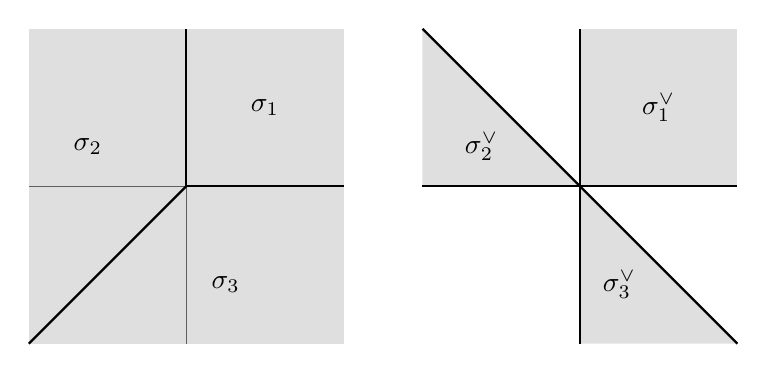
\begin{tikzpicture}
        \begin{scope}
            % Axes
            \draw (-2, 0) -- (2, 0);
            \draw (0, -2) -- (0, 2);
            % Faces
            \fill[fill=gray!50, opacity=0.5] (-2, -2) -- (2, -2) -- (2, 2) -- (-2, 2);
            % Liens
            \draw[thick] (0, 0) -- (2, 0);
            \draw[thick] (0, 0) -- (0, 2);
            \draw[thick] (0, 0) -- (-2, -2);
            % Nodes
            \node at (1, 1) {$\sigma_1$};
            \node at (-1.25, 0.5) {$\sigma_2$};
            \node at (0.5, -1.25) {$\sigma_3$};
        \end{scope}
        \begin{scope}[shift={(5, 0)}]
            % Axes
            \draw (-2, 0) -- (2, 0);
            \draw (0, -2) -- (0, 2);
            % Faces
            \fill[fill=gray!50, opacity=0.5] (0, 0) -- (2, 0) -- (2, 2) -- (0, 2);
            \fill[fill=gray!50, opacity=0.5] (0, 0) -- (-2, 0) -- (-2, 2);
            \fill[fill=gray!50, opacity=0.5] (0, 0) -- (0, -2) -- (2, -2);
            % Liens
            \draw[thick] (-2, 0) -- (2, 0);
            \draw[thick] (0, -2) -- (0, 2);
            \draw[thick] (-2, 2) -- (2, -2);
            % Nodes
            \node at (1, 1) {$\sigma_1^\vee$};
            \node at (-1.25, 0.5) {$\sigma_2^\vee$};
            \node at (0.5, -1.25) {$\sigma_3^\vee$};
        \end{scope}
    \end{tikzpicture} \]
    One computes
    \[ U_{\sigma_1} = \Spec(k[x, y]), \quad U_{\sigma_2} = \Spec(k[x^{-1}, yx^{-1}]), \quad U_{\sigma_3} = \Spec(k[y^{-1}, xy^{-1}]) , \]
    and gluing gives $X(\Delta) \isom \PP_k^2$.

    Conversely, given a toric variety $X$ with torus $T$, one construct a fan $\Delta \subset N_\RR$ with $N = \Hom(\GG_m, T)$ the lattice of one-parameter subgroups and $M = \Hom(T, \GG_m)$ the character lattice of $T$. For any one-parameter subgroup $\lambda : \GG_m \to T$, denote by $\lim_{t \to 0} \lambda(t)$ the limit point in $X$ if it exists. Partitioning $N_\RR$ based on the limit points yields a fan $\Delta$ (after taking closures), such that the corresponding toric variety $X(\Delta)$ is isomorphic to $X$.

    In the example of $X = \PP^2_k$ with maximal torus $T = \GG_m^2$, the one-parameter subgroups of $T$ are given by $\lambda^{a, b}(t) = (t^a, t^b)$ for $a, b \in \ZZ$. The limit points are
    \[ \lim_{t \to 0} \lambda^{a, b}(t) = \left\{ \begin{array}{cl}
        (0 : 0 : 1) & \textup{ if } a, b > 0, \\
        (1 : 0 : 0) & \textup{ if } a < 0 \textup{ and } a < b, \\
        (0 : 1 : 0) & \textup{ if } b < 0 \textup{ and } a > b, \\
        (1 : 0 : 1) & \textup{ if } a = 0 \textup{ and } b > 0, \\
        (0 : 1 : 1) & \textup{ if } b = 0 \textup{ and } a > 0, \\
        (1 : 1 : 0) & \textup{ if } a = b < 0, \\
        (1 : 1 : 1) & \textup{ if } a = 0 = 0.
    \end{array} \right. \]
    Indeed, this corresponds to the fan as given above.
\end{example}

\begin{example}{toric-variety}
    Projective space $\PP^n$ is a toric variety, since the torus
    \[ T = \{ (1 : t_1 : t_2 : \cdots : t_n) : t_i \ne 0 \} \subset \PP^n \]
    is open and dense, and the action of $T$ on itself extends to $\PP^n$ via
    \[ T \times \PP^n \to \PP^n, \quad \left( (t_1, \ldots, t_n), (x_0 : x_1 : \cdots x_n) \right) \mapsto (x_0 : t_1 x_1 : \cdots t_n x_n) . \]
\end{example}

\begin{topic}{formal-completion}{formal completion}
    Let $X$ be a \tref{noetherian-scheme}{noetherian} \tref{scheme}{scheme}, and $Y \subset X$ a \tref{closed-immersion}{closed subscheme}, defined by a \tref{sheaf-of-ideals}{sheaf of ideals} $\mathcal{I}$. The \textbf{formal completion} of $X$ along $Y$, denoted $(\hat{X}, \mathcal{O}_{\hat{X}})$, is the \tref{ringed-space}{locally ringed space} whose topological space $\hat{X}$ is the topological space of $Y$, and $\mathcal{O}_{\hat{X}}$ is the \tref{CT:inverse-limit}{inverse limit} $\varprojlim_n \mathcal{O}_X / \mathcal{I}^n$.
    
    When $X = \Spec R$ is an \tref{affine-scheme}{affine scheme} and $I \subset R$ an ideal, the formal completion is also known as the \textbf{formal spectrum} of $R$ along $I$, denoted $\textup{Spf}(R)$.
\end{topic}

\begin{example}{formal-completion}
    Let $k$ be a field and consider $X = \Spec k[x]$ with closed subscheme $Y \subset X$ given by the ideal $(x)$. Then the formal completion $\hat{X}$ has a topological space consisting of one point, with sheaf of rings given by $\mathcal{O}_{\hat{X}}(\hat{X}) = k \llbracket x \rrbracket$.
    
    Note that the locally ringed space $\hat{X}$ is not the same as $\Spec k \llbracket x \rrbracket$, whose topological space has two points, given by the prime ideals $(0)$ and $(x)$.
\end{example}

\begin{topic}{noetherian-formal-scheme}{noetherian formal scheme}
    A \textbf{noetherian formal scheme} is a \tref{ringed-space}{locally ringed space} $(\mathfrak{X}, \mathcal{O}_\mathfrak{X})$, which has a finite open cover $\{ \mathfrak{U}_i \}$ such that for each $i$, the pair $(\mathfrak{U}_i, \mathcal{O}_\mathfrak{X}|_{\mathfrak{U}_i})$ is isomorphic to the \tref{formal-completion}{formal completion} of some \tref{noetherian-scheme}{noetherian scheme} $X$ along a closed subscheme $Y \subset X$.
\end{topic}

\begin{topic}{algebraic-space}{algebraic space}
    Let $S$ be a \tref{scheme}{scheme} in $\textbf{Sch}_\textup{fppf}$. An \textbf{algebraic space} over $S$ is a \tref{CT:presheaf}{presheaf}
    \[ F : (\textbf{Sch}/S)_\textup{fppf}^\textup{op} \to \textbf{Set} \]
    such that
    \begin{itemize}
        \item $F$ is a \tref{CT:sheaf}{sheaf},
        \item the diagonal $\Delta : F \to F \times F$ is \textit{representable}, that is, for every $T \in (\textbf{Sch}/S)_\textup{fppf}$ and $\xi \in (F \times F)(T) = F(T) \times F(T)$ the fiber product $T \times_{(F \times F)} F$ is representable by a scheme,
        \item there exists a scheme $X \in (\textbf{Sch}/S)_\textup{fppf}$ and a representable map $X \to F$ which is surjective and étale. That is, for every $T \in (\textbf{Sch}/S)_\textup{fppf}$ and $\xi \in F(T)$ the map $X \times_F T \to T$ (of schemes) is surjective and \tref{AG:etale-morphism}{étale}.
    \end{itemize}
\end{topic}

\begin{topic}{mordell-weil-theorem}{Mordell--Weil theorem}
    The \textbf{Mordell--Weil theorem} states that for an \tref{abelian-variety}{abelian variety} $A$ and a \tref{NT:number-field}{number field} $K$, the $K$-rational points $A(K)$ form a \tref{GT:finitely-generated-group}{finitely generated} \tref{GT:abelian-group}{abelian} \tref{GT:group}{group}, called the \textbf{Mordell--Weil group}.
\end{topic}

\begin{topic}{ample-invertible-sheaf}{(very) ample invertible sheaf}
    Let $X$ be a \tref{scheme}{scheme} over $S$. An \tref{invertible-sheaf}{invertible sheaf} $\mathcal{L}$ on $X$ is called \textbf{very ample} relative to $S$, if there is an \tref{immersion}{immersion} $i : X \to \PP_S^n$ for some $n$, such that $\mathcal{L} \isom i^*(\mathcal{O}_{\PP_S^n}(1))$.
    
    An invertible sheaf $\mathcal{L}$ on a \tref{noetherian-scheme}{noetherian scheme} $X$ is \textbf{ample} if for every \tref{coherent-sheaf}{coherent sheaf} $\mathcal{F}$ on $X$, there is an integer $n_0 > 0$ such that for every $n \ge n_0$ the sheaf $\mathcal{F} \otimes \mathcal{L}^{\otimes n}$ is generated by its global sections.
\end{topic}

\begin{example}{ample-invertible-sheaf}
    When $X = \Spec R$ is affine, any invertible sheaf is ample, because every (quasi-)coherent sheaf on an affine scheme is generated by its global sections.
\end{example}

\begin{topic}{cech-cohomology}{Čech cohomology}
    Let $X$ be a \tref{TO:topological-space}{topological space}, $\mathcal{U} = \{ U_i \}_{i \in I}$ an open covering of $X$, and $\mathcal{F}$ a \tref{AG:sheaf}{sheaf} on $X$. Put a well-ordering on $I$ and for convenience write $U_{i_0 \cdots i_p}$ for $U_{i_0} \cap \cdots \cap U_{i_p}$.
    
    The \textbf{Čech complex} of $\mathcal{F}$ with respect to $\mathcal{U}$ is the complex
    \[ C^p(\mathcal{U}, \mathcal{F}) = \prod_{i_0 < \cdots < i_p} \mathcal{F}(U_{i_0 \cdots i_p}) \qquad p \ge 0 , \]
    with differential
    \[ d^p : C^p(\mathcal{U}, \mathcal{F}) \to C^{p + 1}(\mathcal{U}, \mathcal{F}) \]
    \[ (d^p \alpha)_{i_0 , \ldots , i_{p + 1}} = \sum_{k = 0}^{p + 1} (-1)^k \alpha_{i_0 , \ldots , \hat{i}_k, \ldots, i_{p + 1}} | _{U_{i_0 \cdots i_{p + 1}}} . \]
    For all $p \ge 0$ the $p$-th \textbf{Čech cohomology group} of $\mathcal{F}$ with respect to $\mathcal{U}$ is the cohomology group
    \[ \hat{H}^p(\mathcal{U}, \mathcal{F}) = H^p(C^\bdot(\mathcal{U}, \mathcal{F})) . \]
\end{topic}

\begin{example}{cech-cohomology}
    Note that 
    \[ d^0 : C^0(\mathcal{U}, \mathcal{F}) = \prod_{i \in I} \mathcal{F}(U_i) \to C^1(\mathcal{U}, \mathcal{F}) = \prod_{i < j} \mathcal{F}(U_{ij}) \]
    sends $s = (s_i)_{i \in I}$ to $d^0 s = \left(s_j|_{U_i} - s_i|_{U_j}\right)_{ij}$. Therefore, by the sheaf property $\hat{H}^0(\mathcal{U}, \mathcal{F}) = \ker d^0 \isom \mathcal{F}(X)$.
    % H^1 isomorphic to line bundles that trivialize on each U_i
\end{example}

\begin{topic}{sheaf-differentials}{sheaf of differentials}
    Let $f : X \to Y$ be a morphism of \tref{scheme}{schemes}. Covering $X$ and $Y$ by affine opens $V = \Spec A \subset Y$ and $U = \Spec B \subset X$ such that $f(U) \subset V$, consider the sheaf $\widetilde{\Omega_{B/A}}$ on $U$, the sheaf \tref{sheaf-associated-to-module}{associated} to the module \tref{AA:derivation}{$\Omega_{B/A}$}. Gluing these sheaves together gives $\Omega_{X/Y}$, the \textbf{relative sheaf of differentials}.
    
    Alternatively, consider the diagonal morphism $\Delta_{X/Y} : X \to X \times_Y X$, and view $X \xrightarrow{\sim{}} \Delta(X)$ as a \tref{closed-immersion}{closed subscheme} of an open subset $W$ of $X \times_Y X$, with corresponding sheaf of ideals $\mathcal{I}$. Then
    \[ \Omega_{X/Y} = \Delta_{X/Y}^*(\mathcal{I}/\mathcal{I}^2) . \]
\end{topic}

\begin{example}{sheaf-differentials}
    Let $f : X \to Y$ be locally of finite type. If $f$ is \tref{unramified-morphism}{unramified} then $\Omega_{X/Y} = 0$. Namely, since $\Omega_{X/Y}$ behaves well with respect to base change, this can be checked locally, that is, we can assume $Y = \Spec B$ and $X = \Spec A$ with $A \to B$ a local homomorphism of local rings. Using \tref{AA:nakayamas-lemma}{Nakayama's lemma} this reduces to the case where $A$ and $B$ are fields. Being unramified means that $A \subset B$ is a \tref{AA:separable-field-extension}{separable field extension}, and then it is clear that $\Omega_{B/A} = 0$.
    
    Conversely, if $\Omega_{X/Y} = 0$ then $f$ is unramified.
\end{example}

\begin{topic}{albanese-variety}{Albanese variety}
    Let $X$ be a connected \tref{complete-variety}{complete} \tref{variety}{variety} over an algebraically closed field $k$, with a basepoint. Then there exists an \tref{abelian-variety}{abelian variety} $\textup{Alb}(X)$, the \textbf{Albanese variety} of $X$, and a morphism of pointed varieties $i : X \to \textup{Alb}(X)$, the \textbf{Albanese map}, with the universal property that for any other abelian variety $A$ and morphism of pointed varieties $f : X \to A$, there exists a unique morphism of abelian varieties $f' : \textup{Alb}(X) \to A$ such that $f = f' \circ i$.
    \[ \begin{tikzcd} X \arrow{r}{i} \arrow[swap]{dr}{f} &  \textup{Alb}(X) \arrow[dashed]{d}{f'} \\ &  A \end{tikzcd} \]
\end{topic}

\begin{topic}{torsion-sheaf}{torsion sheaf}
    A \textbf{torsion sheaf} is a \tref{sheaf}{sheaf} $\mathcal{F}$ such that $\mathcal{F}(U)$ is a \tref{GT:torsion-group}{torsion} \tref{GT:abelian-group}{abelian group} for every $U$.
\end{topic}

\begin{topic}{flag-variety}{flag variety}
    A \textbf{flag} in a finite-dimensional \tref{LA:vector-space}{vector space} $V$ over a field $k$ is a strictly increasing sequence of subspaces
    \[ 0 = V_0 \subsetneq V_1 \subsetneq \cdots \subsetneq V_m = V . \]
    A flag is \textbf{complete} if $m = \dim V$ and $\dim_k V_i = i$ for all $i$, otherwise it is \textbf{partial}. The \textit{signature} of the flag is the sequence $(d_1, \ldots, d_m)$ where $d_i = \dim_k V_i$.
    
    Given a signature, the set of all flags with such signature is called the \textbf{flag variety} of that signature. It naturally has the structure of a \tref{projective-morphism}{projective} \tref{variety}{variety}.
\end{topic}

\begin{example}{flag-variety}
    The \textit{complete flag variety} (corresponding to signature $(1, \ldots, n)$) is $\textup{GL}_n(k) / B_n(k)$. Namely, all flags are conjugate via base change, and the stabilizer of any given flag is isomorphic to $B_n(k)$, the group of invertible upper triangular matrices.
\end{example}

\begin{example}{flag-variety}
    When $m = 2$, the flag variety parametrizes linear subspaces of $V$. That is, the flag variety is isomorphic to the \tref{LA:grassmannian}{Grassmannian} $\textup{Gr}(d_1, V)$.
\end{example}

\begin{topic}{regular-morphism}{regular morphism}
    Let $f : X \to Y$ be a morphism of \tref{scheme}{schemes}, and assume that all fibers $X_y$ are \tref{noetherian-scheme}{locally noetherian}. Then $f$ is \textbf{regular} at $x \in X$ if $f$ is \tref{flat-morphism}{flat} at $x$ and the fiber $X_{f(x)}$ is \tref{geometrically-regular}{geometrically regular} at $x$ over $k(y)$. The morphism $f$ is \textbf{regular} if it is regular at all points $x \in X$.
\end{topic}

\begin{example}{regular-morphism}
    Every \tref{smooth-morphism}{smooth morphism} is regular, but not conversely. Namely, for any field $k$, the morphism $\Spec k \llbracket t \rrbracket \to \Spec k$ is regular but not smooth, since $k \llbracket t \rrbracket$ is not finitely presented as $k$-algebra. 
\end{example}

\begin{topic}{local-to-global-sequence}{local-to-global Ext sequence}
    Let $X$ be a \tref{scheme}{scheme} and $\mathcal{F}$ and $\mathcal{G}$ \tref{O-module}{$\mathcal{O}_X$-modules}. Then there is a \tref{HA:spectral-sequence}{spectral sequence} (a special case of the \tref{HA:grothendieck-spectral-sequence}{Grothendieck spectral sequence})
    \[ E_2^{p, q} = H^p(X, \mathcal{E}\textup{xt}_X^q(\mathcal{F}, \mathcal{G})) \Rightarrow \textup{Ext}_X^{p + q}(\mathcal{F}, \mathcal{G}) . \]
    In particular, this gives the \textbf{local-to-global Ext sequence}
    \[ 0 \to H^1(X, \mathcal{H}\textup{om}(\mathcal{F}, \mathcal{G})) \to \textup{Ext}_X^1(\mathcal{F}, \mathcal{G}) \to H^0(X, \mathcal{E}\textup{xt}_X^1(\mathcal{F}, \mathcal{G})) \to H^2(X, \mathcal{H}\textup{om}(\mathcal{F}, \mathcal{G})) \to \textup{Ext}_X^2(\mathcal{F}, \mathcal{G}) \]
\end{topic}

\begin{topic}{vector-bundle}{vector bundle}
    A \textbf{vector bundle} is a \tref{free-sheaf}{locally free sheaf} $\mathcal{E}$ of finite rank.
\end{topic}

\begin{topic}{slope-vector-bundle}{slope vector bundle}
    The \textbf{slope} of a \tref{vector-bundle}{vector bundle} $\mathcal{E}$ over a \tref{algebraic-curve}{curve} $C$ is the number $\mu(\mathcal{E}) = \deg \mathcal{E} / \textup{rk} \mathcal{E}$.
\end{topic}

\begin{example}{slope-vector-bundle}
    For any semistable (resp. stable) vector bundle $\mathcal{E}$ and quotient $\mathcal{E} \twoheadrightarrow \mathcal{G}$ we have $\mu(\mathcal{E}) \le \mu(\mathcal{G})$ (resp. $\mu(\mathcal{E}) < \mathcal{G}$). Namely, given an exact sequence $0 \to \mathcal{F} \to \mathcal{E} \to \mathcal{G} \to 0$ we have
    \[ \begin{aligned} \mu(\mathcal{F}) \genfrac{\{}{\}}{0pt}{1}{\le}{<} \mu(\mathcal{E}) &\implies \deg \mathcal{F} \cdot \textup{rk } \mathcal{E} \genfrac{\{}{\}}{0pt}{1}{\le}{<} \deg \mathcal{E} \cdot \textup{rk } \mathcal{F} \\ &\implies \deg \mathcal{G} \cdot \textup{rk } \mathcal{E} \genfrac{\{}{\}}{0pt}{1}{\ge}{>} \deg \mathcal{E} \cdot \textup{rk } \mathcal{G} \implies \mu(\mathcal{G}) \genfrac{\{}{\}}{0pt}{1}{\ge}{>} \mu(\mathcal{E})  , \end{aligned} \]
    since $\deg \mathcal{F} = \deg \mathcal{E} - \deg \mathcal{G}$ and $\textup{rk } \mathcal{F} = \textup{rk } \mathcal{E} - \textup{rk } \mathcal{G}$.
\end{example}

\begin{topic}{stable-vector-bundle}{(semi)stable vector bundle}
    A \tref{vector-bundle}{vector bundle} $\mathcal{E}$ over a \tref{algebraic-curve}{curve} $C$ is \textbf{semistable} (resp. \textbf{stable}) if $\mu(\mathcal{F}) \le \mu(\mathcal{E})$ (resp. $\mu(\mathcal{F}) < \mu(\mathcal{E})$) for every vector subbundle $0 \ne \mathcal{F} \subsetneq \mathcal{E}$, where $\mu(\mathcal{E})$ denotes the \tref{slope-vector-bundle}{slope} of $\mathcal{E}$.
\end{topic}

\begin{topic}{harder-narasimhan-filtration}{Harder--Narasimhan filtration}
    Let $\mathcal{E}$ be a \tref{vector-bundle}{vector bundle} over a \tref{algebraic-curve}{curve} $C$. There exists a unique filtration by subbundles
    \[ 0 = \mathcal{E}_0 \subset \mathcal{E}_1 \subset \cdots \subset \mathcal{E}_{r + 1} = \mathcal{E} \]
    such that $\mathcal{E}_{i + 1}/\mathcal{E}_i$ are \tref{stable-vector-bundle}{semistable vector bundles} with slope $\mu_i$, where $\mu_1 > \mu_2 > \cdots > \mu_r$. This filtration is called the \textbf{Harder--Narasimhan filtration}.
    
    It is constructed as follows. If $\mathcal{E}$ is not semistable, take $0 \ne \mathcal{F} \subsetneq \mathcal{E}$ with maximal \tref{slope-vector-bundle}{slope} and among those with maximal rank. Then $\mathcal{E}_1 := \mathcal{F}$ is semistable by construction, and repeat the process with $\mathcal{E}/\mathcal{F}$.
\end{topic}

\begin{topic}{nef-line-bundle}{nef line bundle}
    A \tref{invertible-sheaf}{line bundle} $\mathcal{L}$ on a \tref{scheme}{scheme} $X$, \tref{proper-morphism}{proper} over a field $k$, is \textbf{nef} (\textit{numerically effective}) if $\deg \mathcal{L}|_C \ge 0$ for every (\tref{closed-immersion}{closed} \tref{TO:irreducible-space}{irreducible}) \tref{algebraic-curve}{curve} $C$ in $X$.
\end{topic}

\begin{topic}{riemann-roch-theorem}{Riemann--Roch theorem}
    Let $C$ be a smooth projective connected \tref{algebraic-curve}{curve} over a field $k$, and $\mathcal{E}$ a \tref{vector-bundle}{vector bundle} over $C$. The \textbf{Riemann--Roch theorem} states that
    \[ \chi(\mathcal{E}) = \dim_k H^0(C, \mathcal{E}) - \dim_k H^1(C, \mathcal{E}) = (1 - g) \textup{rk } \mathcal{E} + \deg \mathcal{E} , \]
    where $g$ is the \tref{geometric-genus}{genus} of $C$ and $\chi(\mathcal{E})$ the \tref{sheaf-euler-characteristic}{Euler characteristic} of $\mathcal{E}$.
\end{topic}

\begin{topic}{algebraic-scheme}{algebraic scheme}
    An \textbf{algebraic scheme} over a field $k$ is a \tref{scheme}{scheme} $X$ over $k$ such that the structure morphism $X \to \Spec k$ is \tref{finite-type}{of finite type}.
\end{topic}

\begin{topic}{projective-variety}{(quasi-)projective variety}
    A \tref{variety}{variety} over a field $k$ is \textbf{projective} if it is isomorphic to a \tref{closed-immersion}{closed} subvariety of some projective space $\PP^n_k$.
    
    A \tref{variety}{variety} over a field $k$ is \textbf{quasi-projective} if it is isomorphic to an open subvariety of a projective variety.
\end{topic}

\begin{topic}{affine-variety}{(quasi-)affine variety}
    A \tref{variety}{variety} over a field $k$ is \textbf{affine} if it is isomorphic to a \tref{closed-immersion}{closed} subvariety of some affine space $\AA^n_k$.
    
    A \tref{variety}{variety} over a field $k$ is \textbf{quasi-affine} if it is isomorphic to an open subvariety of an affine variety.
\end{topic}

\begin{example}{affine-variety}
    The variety $\AA^2 \setminus \{ (0, 0) \}$ is quasi-affine, but not affine.
\end{example}

\begin{topic}{hodge-deligne-polynomial}{Hodge--Deligne polynomial}
    Let $X$ be a \tref{variety}{variety} over $\CC$. The \tref{AT:cohomology-compact-support}{cohomology groups with compact support} $H_c^k(X, \CC)$ naturally carry a \tref{LA:mixed-hodge-structure}{mixed Hodge structure}. The \textbf{Hodge--Deligne polynomial} of $X$ is the polynomial
    \[ \mu(X) = \sum_{k, p, q} h_c^{k; p, q}(X) u^p v^q t^k \in \ZZ[u, v, t] , \]
    where $h_c^{k; p, q}(X) = \dim_\CC \textup{Gr}_F^p \textup{Gr}^W_{p + q} H_c^k(X, \CC)$ are the mixed Hodge numbers.
\end{topic}

\begin{topic}{e-polynomial}{E-polynomial}
    Let $X$ be a \tref{variety}{variety} over $\CC$. The \tref{AT:cohomology-compact-support}{cohomology groups with compact support} $H_c^k(X, \CC)$ naturally carry a \tref{LA:mixed-hodge-structure}{mixed Hodge structure}. The \textbf{$E$-polynomial} of $X$ is the polynomial
    \[ e(X) = \sum_{k, p, q} (-1)^k h_c^{k; p, q}(X) u^p v^q \in \ZZ[u, v] , \]
    where $h_c^{k; p, q}(X) = \dim_\CC \textup{Gr}_F^p \textup{Gr}^W_{p + q} H_c^k(X, \CC)$ are the mixed Hodge numbers.
\end{topic}

\begin{example}{e-polynomial}
    For a closed subvariety $Z \subset X$ with complement $U = X \setminus Z$, there is a long exact sequence of mixed Hodge structures
    \[ \cdots \to H_c^i(U, \CC) \to H_c^i(X, \CC) \to H_c^i(Z, \CC) \to H_c^{i + 1}(U, \CC) \to \cdots \]
    which shows that
    \[ e(X) = e(Z) + e(U) . \]
    Moreover, it can be shown that $e(X \times_\CC Y) = e(X) e(Y)$. This shows that $e : \textbf{Var}_\CC \to \ZZ[u, v]$ factors through the \tref{grothendieck-ring-of-varieties}{Grothendieck ring of varieties}.
\end{example}

\begin{topic}{grothendieck-ring-of-varieties}{Grothendieck ring of varieties}
    Let $S$ be a \tref{variety}{variety} over a field $k$. The \textbf{Grothendieck ring of varieties} over $S$, denoted $\textup{K}(\textbf{Var}/S)$, is defined as the quotient of the \tref{GT:free-group}{free abelian group} on the isomorphism classes of varieties over $S$, by relations of the form
    \[ [X] = [Z] + [U] , \]
    where $Z \subset X$ is a closed subvariety and $U = X \setminus Z$ its open complement. Multiplication is defined by
    \[ [X] \cdot [Y] = [(X \times_S Y)_\textup{red}] \]
    and extended linearly.
\end{topic}

\begin{example}{grothendieck-ring-of-varieties}
    \begin{itemize}
        \item Denote by $\mathbb{L}$ the class of the affine line $\AA^1_k$. Then $[\AA^n_k] = \mathbb{L}^n$.
        \item From the relation $\PP^n_k \setminus \PP^{n - 1}_k \cong \AA^n_k$ one shows inductively that $[\PP^n_k] = \mathbb{L}^n + \cdots + \mathbb{L} + 1$ for all $n > 0$.
        \item Consider the variety $\textup{SL}_2 = \Spec k[a, b, c, d] / (ad - bc - 1)$. Then
        \[ \def\arraystretch{1.5}
        \begin{array}{ccccc}
            [\textup{SL}_2] & = & [\{ (a, b, c, d) \in \AA^4_k \mid a = 0, \; bc = -1 \}] & + & [\{ (a, b, c, d) \in \AA^4_k \mid a \ne 0, \; d = (1 + bc) / a \}] \\
                & = & \mathbb{L} (\mathbb{L} - 1) & + & \mathbb{L}^2 (\mathbb{L} - 1) \\
                & = & \mathbb{L}^3 - \mathbb{L} . &
        \end{array} \]
    \end{itemize}
    
\end{example}

\begin{topic}{excellent-scheme}{(quasi-)excellent scheme}
    A \tref{scheme}{scheme} $X$ is \textbf{(quasi-)excellent} if it has an affine open cover by schemes $\Spec R_i$ with $R_i$ an \tref{AA:excellent-ring}{(quasi-)excellent} ring.
\end{topic}

\begin{topic}{genus-degree-formula}{genus-degree formula}
    Let $C \subset \PP^2$ be a \tref{smooth-morphism}{smooth} \tref{projective-variety}{projective} \tref{algebraic-curve}{curve} given by a homogeneous polynomial of degree $d$. The \textbf{genus-degree formula} expresses the \tref{geometric-genus}{genus} $g$ of $C$ in terms of $d$,
    \[ g = \frac{1}{2}(d - 1)(d - 2) . \]
\end{topic}

\begin{example}{genus-degree-formula}
    Let $E \subset \PP^2$ be given by $Y^2Z - X^3 + XZ^2 = 0$ (of degree $3$), then the genus of $E$ is $\frac{1}{2}(d - 1)(d - 2) = 1$.
\end{example}

\begin{topic}{elliptic-curve}{elliptic curve}
    An \textbf{elliptic curve} is a \tref{smooth-morphism}{smooth} \tref{projective-variety}{projective} \tref{algebraic-curve}{algebraic curve} $E$ over a field $k$ of \tref{geometric-genus}{genus} one, together with a specified point $O$ on $E$. An elliptic curve comes naturally with a group structure, making it an \tref{abelian-variety}{abelian variety}, where $O$ is the unit of the group structure.
\end{topic}

\begin{topic}{fano-variety}{Fano variety}
    A \textbf{Fano variety} is a \tref{complete-variety}{complete variety} whose anti-\tref{canonical-sheaf}{canonical sheaf} $\omega_X^\vee$ is \tref{ample-invertible-sheaf}{ample}.
\end{topic}

\begin{topic}{del-pezzo-surface}{del Pezzo surface}
    A \textbf{del Pezzo surface} is a two-dimensional \tref{fano-variety}{Fano variety}.
\end{topic}

\begin{topic}{kodaira-dimension}{Kodaira dimension}
    Let $X$ be a \tref{projective-variety}{projective variety} over a field $k$. The \textbf{Kodaira dimension} $\kappa(X)$ of $X$ is the \tref{AA:transcendence-degree}{transcendence degree} over $k$ of the ring
    \[ \bigoplus_{n \ge 0} H^0(X, \omega_X^{\otimes n}) \]
    minus $1$, where $\omega_X$ is the \tref{canonical-sheaf}{canonical sheaf} of $X$.
\end{topic}

\begin{topic}{rational-curve}{rational curve}
    A \textbf{rational curve} is an \tref{algebraic-curve}{algebraic curve} which is \tref{birational-map}{birationally equivalent} to the projective line.
\end{topic}

\begin{topic}{zariski-main-theorem}{Zariski's main theorem}
    \textbf{Zariski's main theorem} states that any \tref{separated-morphism}{separated} \tref{quasi-finite-morphism}{quasi-finite} morphism $f : Y \to X$ with $X$ \tref{quasi-compact-scheme}{quasi-compact}, factors as $f' \circ g$, where $f' : Y \to Y'$ is an \tref{open-immersion}{open immersion} and $g : Y' \to X$ is a \tref{finite-morphism}{finite morphism}.
\end{topic}

\begin{topic}{brauer-group}{Brauer group}
    Let $X$ be a \tref{scheme}{scheme}. The \textbf{Brauer group} of $X$ is the second étale cohomology group
    \[ \textup{Br}(X) = H^2_\textup{ét}(X, \GG_m) . \]
\end{topic}

\begin{topic}{rationally-connected-variety}{rationally connected variety}
    A \textbf{rationally connected variety} is a \tref{projective-variety}{projective variety} $X$ over an \tref{AA:algebraically-closed-field}{algebraically closed field} $k$ such that through every two points passes the image of a morphism $\gamma : \PP^1_k \to X$.
\end{topic}

\begin{topic}{quasi-affine-scheme}{quasi-affine scheme}
    A \tref{scheme}{scheme} is \textbf{quasi-affine} if it is \tref{quasi-compact-scheme}{quasi-compact} and isomorphic to an open subscheme of an \tref{affine-scheme}{affine scheme}.
\end{topic}

\begin{topic}{hasse-weil-zeta-function}{Hasse--Weil zeta function}
    Let $X$ be a \tref{variety}{variety} over a finite field $\FF_q$. The \textbf{Hasse--Weil zeta function} of $X$ is given by
    \[ Z(X, t) = \exp \left( \sum_{n = 1}^{\infty} |X(\FF_{q^n})| \frac{t^n}{n} \right) \in \QQ \llbracket t \rrbracket . \]
\end{topic}

\begin{example}{hasse-weil-zeta-function}
    For $X = \PP^m$, we have $|X(\FF_{q^n})| = \sum_{j = 0}^{m} q^{jn}$ for all $n$, so
    \[ Z(\PP^m, t) = \exp \left( \sum_{n = 1}^{\infty} \sum_{j = 0}^{m} \frac{q^{jn} t^n}{n} \right) = \prod_{j = 0}^{m} \frac{1}{(1 - q^j t)} . \]
    In particular,
    \[ Z(\star, t) = \frac{1}{1 - t} \quad \textup{ and } \quad Z(\PP^1, t) = \frac{1}{(1 - t)(1 - qt)} . \]
\end{example}

\begin{example}{hasse-weil-zeta-function}
    The Hasse--Weil zeta function has many different expressions. For $r \ge 1$, let $a_r$ be the number of closed points of $X$ of degree $r$. Then,
    \[ \begin{aligned}
        Z(X, t)
            &= \exp \left( \sum_{n \ge 1} \frac{|X(\FF_{q^n})|}{n} t^n \right) \\
            &= \exp \left( \sum_{n \ge 1} \sum_{r | n} \frac{r \cdot a_r}{n} t^n \right) \\
            &= \exp \left( \sum_{r \ge 1} a_r \sum_{\ell \ge 1} \frac{t^{\ell r}}{\ell} \right) \\
            &= \exp \left( \sum_{r \ge 1} - a_r \log (1 - t^r) \right) \\
            &= \prod_{r \ge 1} (1 - t^r)^{-a_r} \\
            &= \prod_{x \in X_{\textup{cl}}} (1 + t^{\deg(x)} + t^{2 \deg(x)} + \cdots) \\
            &= \sum_{\alpha} t^{\deg(\alpha)} ,
    \end{aligned}\]
    where $\alpha$ runs over the set of effective $0$-cycles on $X$.
\end{example}

\begin{topic}{kapranov-zeta-function}{Kapranov zeta function}
    Let $X$ be a \tref{projective-variety}{quasi-projective variety} over a field $k$. The \textbf{Kapranov zeta function} of $X$ is given by
    \[ Z(X, t) = \sum_{n \ge 0} [\textup{Sym}^n X] t^n \in 1 + t \cdot \textup{K}(\textbf{Var}/k) \llbracket t \rrbracket , \]
    where $\textup{Sym}^n X$ denotes the symmetric product of $X$, that is, the \tref{affine-git-quotient}{GIT quotient} $X^n \sslash S_n$, and $\textup{K}(\textbf{Var}/k)$ denotes the \tref{grothendieck-ring-of-varieties}{Grothendieck ring of varieties}.
    
    For any ring morphism $\mu : \textup{K}(\textbf{Var}/k) \to R$, the \textbf{motivic zeta function} of $X$ is given by
    \[ Z(X, t) = \sum_{n \ge 0} \mu([\textup{Sym}^n X]) t^n \in 1 + t \cdot R \llbracket t \rrbracket . \]
\end{topic}

\begin{example}{kapranov-zeta-function}
    For any closed subvariety $Y \subset X$ with complement $U$, we can identify
    \[ \begin{aligned}
        [\textup{Sym}^n X]
            &= [X^n \sslash S_n] \\
            &= \sum_{i + j = n} [S_n \cdot (Y^i \times U^j) \sslash S_n] \\
            &= \sum_{i + j = n} [Y^i \sslash S_i \times U^j \sslash S_j] \\
            &= \sum_{i + j = n} [ \textup{Sym}^i Y] \cdot [ \textup{Sym}^j U ] ,
    \end{aligned} \]
    and hence
    \[ Z(X, t) = \sum_{n \ge 0} [\textup{Sym}^n X] t^n = \sum_{\substack{n \ge 0 \\ i + j = n}} [\textup{Sym}^i Y] \cdot [\textup{Sym}^j U] t^n = Z(Y, t) \cdot Z(U, t) . \]
    This relation allows to extend the definition of $Z(X, t)$ to all varieties $X$, and, moreover, it gives a group morphism
    \[ Z(-, t) : \textup{K}(\textbf{Var}/k) \to 1 + t \cdot \textup{K}(\textbf{Var}/k) \llbracket t \rrbracket , \]
    with the multiplicative group structure on the right.
\end{example}

\begin{example}{kapranov-zeta-function}
    For $k = \FF_q$ and $\mu : X \mapsto X(\FF_q)$ the point-counting function, the motivic zeta function reduces to the \tref{hasse-weil-zeta-function}{Hasse--Weil zeta function}. Namely, the $\FF_q$-points of $\textup{Sym}^n X$ can be identified with $0$-cycles of degree $n$ on $X$, and the Hasse--Weil zeta function can be expressed as
    \[ Z(X, t) = \sum_{\alpha} t^{\deg(\alpha)} , \]
    where $\alpha$ runs over the set of effective $0$-cycles on $X$.
\end{example}

\begin{example}{kapranov-zeta-function}
    Let $\mathbb{L} = [\AA^1] \in \textup{K}(\textbf{Var}/k)$ be the class of the affine line. By the \tref{AA:symmetric-polynomial}{fundamental theorem of symmetric polynomials}, we have $\operatorname{Sym}^n(\AA^1) \isom \AA^n$ for all $n \ge 0$. More generally, one can show
    \[ Z(\AA^i, t) = 1 + \mathbb{L}^i t + \mathbb{L}^{2i} t^2 + \cdots = \frac{1}{1 - \mathbb{L}^i t} . \]
    In particular,
    \[ Z(\PP^n, t) = Z\left(\bigsqcup_{i = 0}^{n} \AA^i , t\right) = \prod_{i = 0}^{n} Z(\AA^i, t) = \prod_{i = 0}^{n} \frac{1}{1 - \mathbb{L}^i t} . \]
\end{example}

\begin{topic}{luna-slice-theorem}{Luna slice theorem}
    Let $G$ be a \tref{reductive-algebraic-group}{reductive} \tref{algebraic-group}{algebraic group}, acting on an \tref{affine-variety}{affine variety} $X$, over an \tref{AA:algebraically-closed-field}{algebraically closed field} $k$ of characteristic zero. Let $x \in X(k)$ be a smooth point, with \tref{GT:stabilizer}{stabilizer} $G_x$, whose \tref{GT:orbit}{orbit} $O_x$ is closed. Then \textbf{Luna's slice theorem} states that there exists a smooth affine subvariety $Y \subset X$ containing $x$, invariant under $G_x$, such that
    \begin{enumerate}[(i)]
        \item the \tref{tangent-sheaf}{tangent space} at $x$ decomposes as $\mathcal{T}_{X, x} = \mathcal{T}_{Y, x} \oplus \mathcal{T}_{O_x, x}$,
        \item the $G$-equivariant map
        \[ \psi : G \times_{G_x} Y \to X, \quad (g, y) \mapsto g \cdot y , \]
        is \tref{etale-morphism}{étale}, and its image $U$ is open in $X$,
        \item the map
        \[ Y/G_x \isom (G \times_{G_x} Y) / G \xrightarrow{\psi / G} U / G \]
        is étale at $[x]$,
        \item the maps $\psi$ and $G \times_{G_x} Y \to (G \times_{G_x} Y) / G \to Y / G_x$ induce an isomorphism
        \[ G \times_{G_x} Y \isom U \times_{U/G} (Y/G_x) . \]
    \end{enumerate}
    The subvariety $Y$ is called an \textit{étale slice} at $x$.
\end{topic}

\begin{topic}{weighted-projective-space}{weighted projective space}
    Let $k$ be a \tref{AA:ring}{commutative ring}. A \textbf{weighted projective space} over $k$ is the \tref{projective-variety}{projective variety}
    \[ \PP_k(a_0, \ldots, a_n) = \textup{Proj}(k[x_0, \ldots, x_n]) , \]
    with $\deg(x_i) = a_i$, for integers $a_i \in \ZZ$.
\end{topic}

\begin{topic}{moduli-space}{moduli space}
    Let $F : \textbf{Sch}^\textup{op} \to \textbf{Set}$ be a \tref{CT:functor}{functor}.
    A scheme $M$ is a \textbf{fine moduli space} for $F$ if $M$ \tref{CT:representable-functor}{represents} $F$, that is, there is a \tref{CT:natural-transformation}{natural} isomorphism
    \[ F \isom \Hom_\textbf{Sch}(-, M) . \]
    A scheme $M$ is a \textbf{coarse moduli space} for $F$ if there exists a natural transformation
    \[ F \Rightarrow \Hom_\textbf{Sch}(-, M) , \]
    which is universal among all such natural transformations.
\end{topic}

\begin{topic}{valuative-criterion}{valuative criterion}
    Let $f : X \to Y$ be a morphism of \tref{scheme}{schemes} over a scheme $S$, and assume $f$ is \tref{finite-type}{of finite type} and \tref{separated-morphism}{quasi-separated}. The \textbf{valuative criterion} states that $f$ is \tref{proper-morphism}{proper} if and only if for every diagram
    \[ \begin{tikzcd}
        \Spec K \arrow{r} \arrow{d} & X \arrow{d}{f} \\ \Spec R \arrow[dashed]{ur} \arrow{r} & Y
    \end{tikzcd} \]
    where $R$ is a \tref{AA:valuation-ring}{valuation ring} and $K$ its \tref{AA:field-of-fractions}{field of fractions}, there exists a unique morphism $\Spec R \to X$ making the diagram commute. If $Y$ is \tref{noetherian-scheme}{locally noetherian}, it suffices to check the criterion for \tref{AA:discrete-valuation-ring}{discrete valuation rings} $R$.
    
    More precisely, the existence of the dashed arrow corresponds to $f$ being \tref{TO:universally-closed}{universally closed}, and the uniqueness corresponds to $f$ being \tref{separated-morphism}{separated}.
\end{topic}

\begin{example}{valuative-criterion}
    The valuative criterion for properness can be used to show that the morphism $f : \AA^1_k \to \Spec k$ is not proper. Namely, take $R = k[t]_{(t)}$ with $K = k(t)$. Considering the diagram with $\AA^1_k \to \Spec K$ given by $k[x] \to k(t)$, $x \mapsto 1/t$, there does not exist a map $k[x] \to k[t]_{(t)}$ completing the diagram.
\end{example}

\begin{example}{valuative-criterion}
    The valuative criterion for properness can be used to show that the morphism $f : \PP^n \to \Spec \ZZ$ is proper. It can be assumed that $R$ is a discrete valuation ring. A morphism $\Spec K \to \PP^n$ can be expressed in terms of homogeneous coordinates $(a_0 : a_1 : \ldots : a_n)$, with $a_i \in K$ not all zero. Let $a_\textup{min} = \min \{ a_i : 1 \le i \le n, a_i \ne 0 \}$ with respect to the valuation of $R$. Then the $R$-point of $\PP^n$ we are looking for is given by
    \[ \left( \frac{a_0}{a_\textup{min}} : \frac{a_1}{a_\textup{min}} : \ldots : \frac{a_n}{a_\textup{min}} \right) . \]
    Indeed, we have $\frac{a_i}{a_\textup{min}} \in R$ since the valuation is positive, and the coordinates do not vanish simultaneously, since in particular $\frac{a_\textup{min}}{a_\textup{min}} = 1$.
    
    Moreover, since being proper is stable under base change, this shows $\PP^n_X \to X$ is proper for all base schemes $X$.
\end{example}

\begin{topic}{git-fan}{GIT fan}
    Let $G$ be a \tref{reductive-algebraic-group}{reductive algebraic group} acting on a \tref{normal-scheme}{normal} \tref{projective-variety}{projective variety}. In the context of \tref{projective-git-quotient}{GIT quotients}, there is no canonical choice of \tref{equivariant-sheaf}{$G$-linearized} \tref{invertible-sheaf}{invertible sheaf} $\mathcal{L}$ on $X$, and different choices yield different quotients. The GIT fan describes these variations.
    
    Let $\textup{NS}^G(X)$ be the \textit{$G$-Néron--Severi group}, $\textup{NS}^G(X)_\RR = \textup{NS}^G(X) \otimes \RR$, and $\textup{NS}^G(X)_\RR^+$ the convex cone generated by \tref{ample-invertible-sheaf}{ample} $G$-linearized invertible sheaves, and
    \[ C^G(X) = \{ \ell \in \textup{NS}^G(X)_\RR^+ \mid X^\textup{ss}(\ell) \ne \varnothing \} \subset \textup{NS}^G(X)_\RR^+ \]
    the cone of \textit{effective points}.
    
    Then, for all $\ell \in C^G(X)$, the subsets
    \[ C(\ell) = \{ \ell' \in C^G(X) \mid X^\textup{ss}(\ell') = X^\textup{ss}(\ell) \} \]
    are closed convex \tref{LA:polyhedral-cone}{rational polyhedral cones} in $C^G(X)$, and together they form a \tref{LA:fan}{fan} covering $C^G(X)$. This fan is called the \textbf{GIT fan} for the action of $G$ on $X$.
\end{topic}

\begin{topic}{relative-spectrum}{relative spectrum}
    Let $S$ be a \tref{scheme}{scheme} and $\mathcal{A}$ a \tref{coherent-sheaf}{quasi-coherent} \tref{O-algebra}{sheaf of $\mathcal{O}_S$-algebras}. For any cover of $S$ by affine opens $\{ U_i \}$, the natural maps $\mathcal{O}_S(U_i) \to \mathcal{A}(U_i)$ induce morphisms $\pi_i : \Spec(\mathcal{A}(U_i)) \to U_i$, which glue together to a scheme
    \[ \pi : \underline{\Spec}_S(\mathcal{A}) \to S , \]
    called the \textbf{relative spectrum} of $\mathcal{A}$.
\end{topic}

\begin{topic}{spreading-out}{spreading-out}
    Let $X$ be a \tref{variety}{variety} over $\CC$. A \textbf{spreading-out} of $X$ is a \tref{separated-scheme}{separated} scheme $\tilde{X}$ over a \tref{AA:finitely-generated-algebra}{finitely generated $\ZZ$-algebra} $R$ with an embedding $R \to \CC$, such that $X \isom \tilde{X} \times_R \CC$.
\end{topic}

\begin{example}{spreading-out}
    Let $X \subset \AA^n_\CC$ be an affine variety defined by polynomials $f_1, \ldots, f_r \in \CC[x_1, \ldots, x_n]$. Writing $f_i = \sum_{j, k} a_{ijk} x_j^k$, we see that a spreading-out $\tilde{X}$ can be defined over $R = \ZZ[a_{ijk}]$ by the same polynomials $f_i$, from which it is clear that $X \isom \tilde{X} \times_R \CC$.
\end{example}

% \begin{topic}{mixed-hodge-polynomial}{mixed Hodge polynomial}
%     Let $X$ be a complex \tref{variety}{variety}. Deligne showed the \tref{AT:cohomology-compact-support}{compactly supported cohomology groups} $H_c^k(X; \QQ)$ naturally carry a \tref{UN:mixed-hodge-structure}{mixed Hodge structure}. The \textbf{mixed Hodge polynomial} of $X$ is the polynomial
%     \[ H_c(X) = \sum_{p, q, k} h_c^{k; p, q}(X) u^p v^q t^k \in \ZZ[u, v, t] . \]
% \end{topic}

\begin{topic}{blowup}{blowup}
    Let $X$ be a \tref{scheme}{scheme} and $Z \subset X$ a \tref{closed-immersion}{closed subscheme} given by a \tref{sheaf-of-ideals}{sheaf of ideals} $\mathcal{I} \subset \mathcal{O}_X$. A \textbf{blowup} of $X$ along $Z$ is a morphism of schemes
    \[ \pi : \textup{Bl}_Z(X) \to X \]
    with the universal property that for every morphism $f : Y \to X$ such that $f^* \mathcal{I}$ is \tref{invertible-sheaf}{invertible}, there exists a unique morphism $g : Y \to \textup{Bl}_Z(X)$ such that $\pi \circ g = f$.

    When the closed immersion $Z \to X$ is \tref{finite-presentation}{of finite presentation}, a blowup of $X$ along $Z$ exists and is given by
    \[ \textup{Bl}_Z(X) = \underline{\Proj}_X \left( \bigoplus_{n \ge 0} \mathcal{I}^n \right) . \]
\end{topic}

\begin{example}{blowup}
    For any scheme $X$, it follows directly from the universal property that
    \[ \textup{Bl}_\varnothing(X) = X \quad \textup{ and } \quad \textup{Bl}_X(X) = \varnothing . \]
\end{example}

\begin{example}{blowup}
    Let $X \subset \AA^n_k$ be an \tref{affine-variety}{affine variety}, and $Z \subset X$ a closed subvariety given by the vanishing locus of $f_1, \ldots, f_r \in \mathcal{O}_X(X)$. Writing
    \[ f : (X \setminus Z) \to \PP^{r - 1}, \quad x \mapsto (f_1(x) : \cdots : f_r(x)) , \]
    the blowup of $X$ at $Z$ is the closure of the graph $\Gamma_f \subset X \times \PP^{r - 1}$,
    \[ \pi : \textup{Bl}_Z(X) := \overline{\Gamma}_f \to X . \]

    In particular, consider the following examples:
    \begin{itemize}
        \item Consider the cusp $C$ in the affine plane given by $y^2 - x^3 = 0$. Blowing up at the origin $(0, 0)$, i.e. the ideal $(x, y)$, gives
        \[ \textup{Bl}_{\{ (0, 0) \}}(C) = \overline{\{ ((x, y), (u : v)) \in (C \setminus \{ (0, 0) \}) \times \PP^1 \mid xv = uy \}} . \]
        We can cover this blowup by two affine charts
        \[ U_x = \{ \tilde{y}^2 - x = 0, \; y = \tilde{y} x \}, \qquad U_y = \{ y - \tilde{x}^3 = 0, \; x = \tilde{x} y \} \]
        with the obvious transition maps and projection maps to $C$.
        
        \item Consider \textit{Whitney's umbrella} $W = \{ x^2 - y^2 z = 0 \} \subset \AA^3_k$. The blowup of $W$ in the origin $(0, 0, 0)$ can be described by the charts
        \[ \begin{aligned}
            U_x = \{ 1 - x \tilde{y}^2 \tilde{z}, \; y = \tilde{y} x, \; z = \tilde{z} x \} , \\
            U_y = \{ \tilde{x}^2 - y \tilde{z}, \; x = \tilde{x} y, \; z = \tilde{z} y \} , \\
            U_z = \{ \tilde{x}^2 - \tilde{y}^2 z, \; x = \tilde{x} z, \; y = \tilde{y} z \}
        \end{aligned} \]
        In particular, in $U_z$ we find the same singularity as in $W$. However, blowing up in the $z$-axis gives
        \[ U_x = \{ 1 - \tilde{y}^2 z, \; y = \tilde{y} x \}, \qquad U_y = \{ \tilde{x}^2 - z, \; x = \tilde{x} y \} . \]
    \end{itemize}
\end{example}

\begin{topic}{strict-transform}{strict transform}
    Let $X$ be a \tref{scheme}{scheme} with \tref{closed-immersion}{closed subscheme} $Z \subset X$ and \tref{blowup}{blowup} $\pi : \textup{Bl}_Z(X) \to X$. The \textbf{strict transform} of a closed subscheme $Y \subset X$ is the closure of $\pi^{-1}(Y \setminus Z)$ inside $\textup{Bl}_Z(X)$.
\end{topic}

\begin{topic}{resolution-of-singularities}{resolution of singularities}
    Let $X$ be a \tref{variety}{variety}. A \textbf{resolution of singularities} of $X$ is a \tref{proper-morphism}{proper} \tref{birational-map}{birational morphism} $\widetilde{X} \to X$, where $\widetilde{X}$ is a \tref{non-singular-variety}{non-singular variety}.
\end{topic}

\begin{topic}{non-singular-variety}{non-singular variety}
    A \tref{variety}{variety} $X$ over a field $k$ is \textbf{non-singular at a point $x \in X$} if the local ring $\mathcal{O}_{X, x}$ is \tref{AA:regular-ring}{regular}. The variety $X$ is \textbf{non-singular} if it is non-singular at all points $x \in X$.
    
    Equivalently, $X$ is non-singular if and only if the structure morphism $X \to \Spec k$ is \tref{smooth-morphism}{smooth}.
\end{topic}

\begin{topic}{chow-lemma}{Chow's lemma}
    % Let $S$ be a \tref{noetherian-scheme}{noetherian} \tref{scheme}{scheme}, and $X$ a scheme \tref{proper-morphism}{proper} over $S$. Then \textbf{Chow's lemma} states that there exists a scheme $X'$ which is \tref{projective-morphism}{projective} over $S$, and a surjective morphism $f : X' \to X$ over $S$, which induces an isomorphism $f^{-1}(U) \isom U$ for some \tref{TO:dense}{dense} open $U \subset X$.
    Let $S$ be a \tref{noetherian-scheme}{noetherian} \tref{scheme}{scheme}, and $f : X \to S$ a \tref{separated-morphism}{separated morphism} of \tref{finite-type}{finite type}. Then \textbf{Chow's lemma} states that there exists a commutative diagram
    \[ \begin{tikzcd}
        X \arrow[swap]{dr}{f} & X' \arrow[swap]{l}{\pi} \arrow{r}{i} \arrow{d} & \PP^n_S \arrow{dl} \\ & S &
    \end{tikzcd} \]
    with $\pi : X' \to X$ \tref{proper-morphism}{proper} and surjective, $i : X' \to \PP^n_S$ an \tref{immersion}{immersion}, such that $\pi$ restricts to an isomorphism $\pi^{-1}(U) \isom U$ for some \tref{TO:dense-set}{dense} open $U \subset X$.
 \end{topic}

\begin{topic}{normal-crossings-divisor}{normal crossings divisor}
    Let $X$ be a \tref{scheme}{scheme} over a base scheme $S$. A \textbf{normal crossings divisor} of $X$ is a \tref{closed-immersion}{closed subscheme} $D$ of $X$ such that for all $x \in X$, there exists an integer $n \ge 0$, a scheme $U/S$, an \tref{etale-morphism}{étale morphism} $f : U \to X$ with $x \in f(U)$, and an étale morphism $g : U \to \AA^n_S$, such that $f^* D = g^* Z$, where $Z = V(x_1 x_2 \cdots x_n) \subset \AA^n_S$ is the union of the coordinate hyperplanes.
\end{topic}

\begin{example}{normal-crossings-divisor}
    Let $k$ be a field, $X = \AA^2_k$, and $D = \Spec k[x, y] / (y^2 - x^3 - x)$. Then $D$ is a normal crossings divisor of $X$. In particular, at the point given by the maximal ideal $(x, y)$, take $U = \Spec k[x, y, t, s] / (t^2 - (x + 1), s (x + 1) - 1)$ with $f : U \to X$ the obvious morphism and $g : U \to \AA^2_k = \Spec k[u, v]$ the morphism given by $u \mapsto y - xt$ and $v \mapsto y + xt$. Then
    \[ \begin{aligned}
        f^* D
            &= \Spec k[x, y, t, s] / (t^2 - (x + 1), s(x + 1) - 1, y^2 - x^3 - x) \\
            &= \Spec k[x, y, t, s] / (t^2 - (x + 1), s(x + 1) - 1, (y - xt)(y + xt)) \\
            &= g^* Z ,
    \end{aligned} \]
    where we used that $y^2 - x^3 - x = y^2 - x^2 t^2 = (y - xt)(y + xt)$ over $U$.
\end{example}

\begin{topic}{hasse-weil-bound}{Hasse--Weil bound}
    Let $C$ be a \tref{non-singular-variety}{smooth} \tref{projective-variety}{projective} \tref{algebraic-curve}{curve} over a finite field $\FF_q$ of \tref{geometric-genus}{genus} $g$. The \textbf{Hasse--Weil bound} states that
    \[ | \#C(\FF_q) - q - 1 | \le 2 g \sqrt{q} . \]
\end{topic}

\begin{topic}{analytification}{analytification}
    Let $X$ be a \tref{non-singular-variety}{non-singular} \tref{variety}{variety} over $\CC$. 
    The set of complex points $X(\CC)$ naturally has a \tref{TO:topological-space}{topology}, such that for any affine open $U \subset X$ the topology on $U(\CC) \subset \CC^n$ is given by the \tref{TO:subspace-topology}{subspace topology} of the Euclidean topology on $\CC^n$. These charts give $X(\CC)$ the structure of a \tref{DG:complex-manifold}{complex manifold} $X^\textup{an}$, called the \textbf{analytification} of $X$. Moreover, a morphism of non-singular complex varieties $f : X \to Y$ induces a holomorphic map $f^\textup{an} : X^\textup{an} \to Y^\textup{an}$, and this construction yields the \textit{analytification functor}
    \[ (-)^\textup{an} : \textbf{SmVar}_\CC \to \textbf{Mfld}_\CC . \]
\end{topic}

\begin{topic}{etale-fundamental-group}{étale fundamental group}
    Let $X$ be a \tref{scheme}{scheme} over a field $k$, and let $\overline{x} \to X$ be a \tref{geometric-point}{geometric point} of $X$. Let $\textbf{FÉt}/X$ be the category of \tref{finite-morphism}{finite} \tref{etale-morphism}{étale} coverings $\pi : Y \to X$ over $X$. The functor
    \[ F : \textbf{FÉt}/X \to \textbf{Set}, \quad Y \mapsto \Hom_X(\overline{x}, Y) \]
    is \tref{CT:pro-representable-functor}{pro-representable}, meaning there exists a \tref{CT:direct-limit}{direct system} $\tilde{X} = (X_i)_{i \in I}$ in $\textbf{FÉt}/X$ such that $F(Y) = \varinjlim_{i \in I} \Hom_X(X_i, Y)$ functorially in $Y$. Moreover, each $X_i$ can be chosen \tref{galois-cover}{Galois} over $X$, so that the order of $\textup{Aut}_X(X_i)$ equal the degree of $X_i$ over $X$.
    
    The \textbf{étale fundamental group} of $X$ at $\overline{x}$ is the \tref{TO:topological-group}{topological group} given by the \tref{CT:inverse-limit}{inverse limit}
    \[ \pi_1^\textup{ét}(X, \overline{x}) = \varprojlim_{i \in I} \textup{Aut}_X(X_i) , \]
    with the natural topology as an inverse limit of finite discrete groups.
\end{topic}

\begin{example}{etale-fundamental-group}
    For $X = \Spec k$, the functor $F$ is actually representable by $\tilde{X} = \Spec k^\textup{sep}$, where $k^\textup{sep}$ denotes the \tref{AA:separable-closure}{separable closure} of $k$. The étale fundamental group of $X$ is
    \[ \pi_1^\textup{ét}(X, \overline{x}) \cong \operatorname{Aut}_X(\tilde{X}) = \operatorname{Gal}(k^\textup{sep}/k) , \]
    which is the absolute Galois group of $k$.
\end{example}

\begin{example}{etale-fundamental-group}
    Let $X = \AA^1_k \setminus \{ 0 \}$ over $k = \CC$, and take $\overline{x} = 1$. A direct system pro-representing $F$ is given by
    \[ \pi_n : X_n = \AA^1_k \setminus \{ 0 \} \to X, \quad x \mapsto x^n , \]
    for each integer $n \ge 1$, with a morphism $X_m \to X_n$, $x \mapsto x^{m/n}$ whenever $n$ divides $m$. Note that $\textup{Aut}_X(X_n) \isom \ZZ/n\ZZ$, where $k \mod n$ corresponds to the automorphism $X_n \to X_n$ given by $x \mapsto \zeta_n^k x$. The étale fundamental group of $X$ at $\overline{x}$ is now
    \[ \pi_1^\textup{ét}(X, \overline{x}) = \varprojlim_{n \ge 1} \ZZ/n\ZZ = \hat{\ZZ} , \]
    the \tref{GT:profinite-group}{profinite completion} of $\ZZ$.
\end{example}

\begin{topic}{l-adic-cohomology}{l-adic cohomology}
    Let $X$ be a \tref{scheme}{scheme} over a field $k$, and $\ell$ a prime number different from the \tref{AA:characteristic}{characteristic} of $k$. The \textbf{$\ell$-adic cohomology} of $X$ is given by the \tref{CT:inverse-limit}{inverse limit}
    \[ H^i(X, \ZZ_\ell) = \varprojlim_{n \in \NN} H^i(X, \ZZ/\ell^n \ZZ) \]
    and
    \[ H^i(X, \QQ_\ell) = H^i(X, \ZZ_\ell) \otimes_{\ZZ_\ell} \QQ_\ell , \]
    where $\ZZ_\ell$ denotes the \tref{NT:p-adic-numbers}{$\ell$-adic integers} and $\QQ_\ell$ its \tref{AA:field-of-fractions}{field of fractions}.
\end{topic}

\begin{topic}{grothendieck-trace-formula}{Grothendieck trace formula}
    Let $X$ be a \tref{variety}{variety} over a finite field $\FF_q$, and let $\overline{X} = X \times_{\FF_q} \overline{\FF}_q$ for an \tref{AA:algebraic-closure}{algebraic closure} $\overline{\FF}_q$ of $\FF_q$. Let $F : \overline{X} \to \overline{X}$ be the morphism induced by the \tref{AA:frobenius-morphism}{Frobenius morphism} $\overline{\FF}_q \to \overline{\FF}_q$ given by $x \mapsto x^q$. The \textbf{Grothendieck trace formula} states that
    \[ \# X(\FF_q) = \sum_{i = 0}^{2 \dim X} \tr(F, H^i_c(\overline{X}, \QQ_\ell)) , \]
    where $F$ naturally acts on the (compactly supported) \tref{l-adic-cohomology}{$\ell$-adic cohomology} of $\overline{X}$.
\end{topic}

\begin{example}{grothendieck-trace-formula}
    Consider $X = \PP^1$ over $\FF_q$. Then
    \[ H^i(\overline{X}, \QQ_\ell) = \left\{ \begin{array}{cl}
        \QQ_\ell & \textup{ if } i = 0, \\
        0 & \textup{ if } i = 1, \\
        \QQ_\ell(-1) & \textup{ if } i = 2, \\
    \end{array} \right. \]
    and
    \[ \tr(F, H^i(\overline{X}, \QQ_\ell)) = \left\{ \begin{array}{cl}
        1 & \textup{ if } i = 0, \\
        0 & \textup{ if } i = 1, \\
        q & \textup{ if } i = 2, \\
    \end{array} \right. \]
    so the Grothendieck trace formula yields
    \[ \# \PP^1(\FF_q) = 1 + q , \]
    as expected.
\end{example}

\begin{topic}{stably-birational}{stably birational}
    Two \tref{variety}{varieties} $X$ and $Y$ over a field $k$ are \textbf{stably birational} if $X \times \PP^m_k$ is \tref{birational-map}{birational} to $Y \times \PP^n_k$ for some $m, n \ge 0$.
\end{topic}

\begin{topic}{larsen-lunts-theorem}{Larsen--Lunts theorem}
    Let $\textup{SB}$ be the set of \tref{stably-birational}{stably birational} equivalence classes of \tref{non-singular-variety}{smooth} \tref{projective-variety}{projective} \tref{variety}{varieties} over $\CC$. The \textbf{Larsen--Lunts theorem} states that there exists a unique ring morphism
    \[ \phi : \textup{K}(\textbf{Var}_\CC) \to \ZZ[\textup{SB}] , \]
    from the \tref{grothendieck-ring-of-varieties}{Grothendieck ring of varieties}, such that $\phi([X])$ is the class of $X$ in $\textup{SB}$ for any smooth proper $X$. Moreover, the kernel of $\phi$ is the ideal generated by $\mathbb{L} = [\AA^1_\CC]$, so that
    \[ \textup{K}(\textbf{Var}_\CC) / (\mathbb{L}) \isom \ZZ[\textup{SB}] . \]
\end{topic}

\begin{topic}{riemann-hurwitz-formula}{Riemann--Hurwitz formula}
    Let $f : C' \to C$ be a morphism between \tref{non-singular-variety}{smooth} \tref{projective-variety}{projective} \tref{algebraic-curve}{curves} $C'$ and $C$. The \textbf{Riemann--Hurwitz formula} states that
    \[ \chi(S') = \deg(f) \cdot \chi(S) - \sum_{P \in S'} (e_P - 1) , \]
    where $\chi$ denotes the \tref{AT:euler-characteristic}{Euler characteristic}, and $e_P$ denotes the ramification index of $f$ at $P$.
\end{topic}

\begin{topic}{unirational-variety}{unirational variety}
    Let $X$ be a \tref{variety}{variety} over a field $k$. Then $X$ is \textbf{unirational} if it is \tref{integral-scheme}{integral} and there is an embedding $k(X) \subset k(x_1, \ldots, x_n)$ of the function field of $X$ into a purely transcendental extension of $k$.
\end{topic}

\begin{topic}{fermat-curve}{Fermat curve}
    A \textbf{Fermat curve} over a field $k$ is a \tref{projective-variety}{projective} \tref{algebraic-curve}{curve} in $\PP^2_k$ given by a homogeneous equation
    \[ X^n + Y^n = Z^n \]
    for some $n \ge 2$.
\end{topic}

% \begin{topic}{motivic-integration}{motivic integration}
%     Let $X$ be a \tref{non-singular-variety}{smooth} complex \tref{variety}{variety} of dimension $n$. Define
%     \[ \begin{array}{cc}
%         \Delta_m = \Spec \CC[t] / (t^{m + 1}), & \Delta_\infty = \Spec \CC \llbracket t \rrbracket \\[10pt]
%         X_m = \Hom_\CC(\Delta_m, X), & X_\infty = \Hom_\CC(\Delta_\infty, X) .
%     \end{array} \]
%     and \textit{truncation maps} $\pi^k_m : X_k \to X_m$ for $k \ge m$ and $\psi_m : X_\infty \to X_m$, induced by the natural maps $\Delta_m \to \Delta_k$ and $\Delta_\infty \to \Delta_m$, respectively.
    
%     For any $C \subset X_\infty$, which can be written as $C = \psi_m^{-1}(C_m)$ for some \tref{TO:constructible-set}{constructible} $C_m \subset X_m$, the \textbf{motivic measure} of $C$ is
%     \[ \mu(C) = \frac{[C_m]}{\mathbb{L}^{n(m + 1)}} \in \textup{K}(\textbf{Var}_\CC)[\mathbb{L}^{-1}] \]
%     as an element in the \tref{grothendieck-ring-of-varieties}{Grothendieck ring of varieties} localized by the Lefschetz motive $\mathbb{L} = [\AA^1_\CC]$.
%     This is well-defined, because if $C = \psi_m^{-1}(C_m) = \psi_k^{-1}(C_k)$ for some $k > m$, then $C_k = (\pi_m^k)^{-1}(C_m)$ is an $\AA_\CC^{n(k - m)}$-bundle over $C_m$, so $[C_k] = [C_m] \cdot \mathbb{L}^{n(k - m)}$.
%     The \textbf{motivic measure} of $X$ is defined as
%     \[ \mu(X) = \mu(X_\infty) = \frac{[X]}{\mathbb{L}^n} . \]
% \end{topic}

\begin{topic}{motivic-integration}{motivic integration}
    Let $X$ be a \tref{non-singular-variety}{smooth} complex \tref{variety}{variety} of dimension $n$. Denote by $J_\infty(X) = \Hom(\Spec(\CC \llbracket t \rrbracket), X)$ the space of \textit{formal arcs} on $X$. For any \tref{weil-divisor}{prime divisor} $D \subset X$, define the function
    \[ F_D : J_\infty(X) \to \ZZ_{\ge 0} \cup \{ \infty \} \]
    that sends a formal arc $\gamma$ to the order of vanishing of the power series $g(\gamma(t))$ at $t = 0$, where $g$ is a local defining equation for $D$ around $\gamma(0) \in X$. For an \tref{weil-divisor}{effective divisor} $D = \sum_{i = 1}^{r} a_i D_i$ with simple normal crossings on $X$, define
    \[ F_D = \sum_{i = 1}^{r} a_i F_{D_i} . \]
    The \textbf{motivic integral} of the pair $(X, D)$ is
    \[ \int_{J_\infty(X)} F_D \; d \mu = \sum_{J \subset \{ 1, \ldots, r \}} \frac{[D_J^\circ]}{\mathbb{L}^n} \prod_{j \in J} \frac{\mathbb{L} - 1}{\mathbb{L}^{a_j + 1} - 1} \]
    as an element in the \tref{AA:completion}{completed} \tref{AA:localization}{localized} \tref{grothendieck-ring-of-varieties}{Grothendieck ring of varieties} $\widehat{\textup{K}(\textbf{Var}_\CC)[\mathbb{L}^{-1}]}$, where $\mathbb{L} = [\AA^1_\CC]$ and $D_J^\circ = \bigcap_{j \in J} D_j \mathbin{\big\backslash} \bigcup_{i \in \{ 1, \ldots, r \} \setminus J} D_i$.

    For a complex variety $X$ with at worst Gorenstein canonical singularities, the \textbf{motivic integral} of $X$ is the motivic integral of $(Y, D)$, where $\varphi : Y \to X$ is any \tref{resolution-of-singularities}{resolution of singularities} for which $D = K_Y - \varphi^* K_X$ has only simple normal crossings.
\end{topic}

\begin{example}{motivic-integration}
    \begin{itemize}
        \item For $X$ a smooth complex variety and $D = 0$, the motivic integral of $(X, D)$ is $[D_\varnothing^\circ] / \mathbb{L}^{\dim X} = [X] / \mathbb{L}^{\dim X}$.
    \end{itemize}
\end{example}

\begin{topic}{nisnevich-morphism}{Nisnevich morphism}
    A morphism $f : X \to Y$ of \tref{scheme}{schemes} is \textbf{Nisnevich} if it is \tref{etale-morphism}{étale} and for every point $y \in Y$, there exists a point $x \in X$ with $f(x) = y$ such that the induced map on residue fields $k(y) \to k(x)$ is an isomorphism.
\end{topic}

\begin{example}{nisnevich-morphism}
    The morphism
    \[ f : \Spec \CC[x^{\pm 1}, y] / (y^2 - x) \to \Spec \CC[x^{\pm 1}] \]
    is étale, but not Nisnevich, because the induced map on residue fields for the generic point
    \[ f^\# : \CC(x) \to \CC(x)[y] / (y^2 - x) \]
    is not an isomorphism. However, if we add $\Spec \CC(x) \to \Spec \CC[x^{\pm 1}]$ to the morphism, then
    \[ \tilde{f} : \Spec \CC[x^{\pm 1}, y] / (y^2 - x) \sqcup \Spec \CC(x) \to \Spec \CC[x^{\pm 1}] , \]
    is Nisnevich.
\end{example}

\begin{topic}{jacobian-variety}{Jacobian variety}
    Let $C$ be a \tref{complete-variety}{complete} \tref{smooth-morphism}{smooth} \tref{algebraic-curve}{curve} over a field $k$, such that $C(k)$ is non-empty.
    The \textbf{Jacobian variety} of $C$ is a variety $J(C)$ over $k$ representing the functor
    \[ T \mapsto \operatorname{Pic}_{X/k}(T)^0 , \]
    where $\operatorname{Pic}_{X/k}$ is the \tref{picard-functor}{relative Picard functor}.
\end{topic}

\begin{example}{jacobian-variety}
    Let $E$ be an \tref{elliptic-curve}{elliptic curve}. Then the Jacobian $J(E)$ of $E$ is isomorphic to $E$ via the isomorphism
    \[ E \xrightarrow{\sim} J(E), \quad P \mapsto \mathcal{O}_E(P - O) , \]
    where $O$ is the unit of the elliptic curve.
\end{example}

\begin{topic}{polarized-variety}{polarized variety}
    A \textbf{polarization} of a \tref{variety}{variety} $X$ over an \tref{AA:algebraically-closed-field}{algebraically closed field} $k$ is a choice of an \tref{ample-invertible-sheaf}{ample line bundle} on $X$, up to \tref{algebraic-equivalence}{algebraic equivalence}.
\end{topic}

\begin{topic}{semi-separated-morphism}{semi-separated morphism}
    A morphism $f : X \to Y$ of \tref{scheme}{schemes} is \textbf{semi-separated} if the diagonal $\Delta_{X/Y} : X \to X \times_Y X$ is \tref{affine-morphism}{affine}.
\end{topic}

\begin{example}{semi-separated-morphism}
    If $f : X \to S$ is a semi-separated morphism with $S$ affine, then intersections of open affines on $X$ are again open affine. That is, for two open affines $U, V \subset X$, their intersection is given by
    \[ U \cap V = U \times_X V = \Delta_{X/S}^{-1}(U \times_S V) , \]
    which is again affine open.
\end{example}

\begin{example}{semi-separated-morphism}
    Any \tref{separated-morphism}{separated morphism} is semi-separated morphism, and any semi-separated morphism is quasi-separated, but the converses do not hold.
    
    Namely, let $X$ be the affine plane with double origin, over a field $k$. Then $X \to \Spec k$ is quasi-compact, but not semi-separated as the intersection of the two affine planes $U, V \subset X$, which is $U \cap V = \AA^2_k \setminus \{ (0, 0) \}$, is not affine.
    
    Furthermore, let $Y$ be the affine line with double origin, over a field $k$. Then $Y \to \Spec k$ is semi-separated, but not separated.
\end{example}

\begin{topic}{function-field}{function field}
    Let $X$ be an \tref{TO:irreducible-space}{irreducible} \tref{variety}{variety} over a field $k$. The \textbf{function field} of $X$ is the field $K(X)$ over $k$ given by
    \[ K(X) = \{ (U, f) : U \subset X \textup{ dense open and } f \in \mathcal{O}_X(U) \} / \sim{} \]
    where $(U, f) \sim{} (V, g)$ if and only if $f|_{U \cap V} = g|_{U \cap V}$.
\end{topic}

\begin{example}{function-field}
    For an affine variety $X = \Spec R$ over $k$, the function field of $X$ is given by the \tref{AA:field-of-fractions}{field of fractions} of $R$.
\end{example}

\begin{topic}{hyperelliptic-curve}{hyperelliptic curve}
    A \textbf{hyperelliptic curve} is an \tref{algebraic-curve}{algebraic curve} over a field $k$ of \tref{geometric-genus}{genus} $g > 1$, given by an equation of the form
    \[ y^2 + h y = f \]
    where $f \in k[x]$ is a \tref{AA:separable-polynomial}{separable polynomial} of degree $n = 2g + 1$ or $n = 2g + 2$, and $h \in k[x]$ is a polynomial of degree less than $g + 2$. When $\operatorname{char}(k) \ne 2$, one can take $h = 0$ by a substitution of variables.
\end{topic}

\begin{topic}{proj-construction}{Proj construction}
    Let $S = \bigoplus_{i \ge 0} S_i$ be a \tref{AA:graded-ring}{graded ring}. The \textbf{Proj construction} assigns to $S$ the \tref{scheme}{scheme} $\Proj S = (X, \mathcal{O}_X)$ defined as follows.
    \begin{itemize}
        \item The topological space $X$ is the set of homogeneous \tref{AA:prime-ideal}{prime ideals} $\mathfrak{p} \subset S$ not containing the irrelevant ideal $S_+ = \bigoplus_{i > 0} S_i$, whose closed sets are given precisely by the sets $V(\mathfrak{a}) = \{ \textup{homogeneous prime ideals } \mathfrak{p} \subset S \textup{ with } \mathfrak{p} \supset \mathfrak{a} \}$ for all homogeneous ideals $\mathfrak{a} \subset S$.
        \item The sheaf of rings $\mathcal{O}_X$ is given as follows. For each open set $U \subset X$, $\mathcal{O}_X(U)$ is the set of functions $s : U \to \sqcup_{\mathfrak{p} \in U} {(S_\mathfrak{p})}_0$ with $s(\mathfrak{p}) \in (S_\mathfrak{p})_0$ for each $\mathfrak{p} \in U$, such that $s$ is locally a quotient of elements in $S$. This means that for each $\mathfrak{p} \in U$, there is a neighborhood $V \subset U$ of $\mathfrak{p}$, and homogeneous elements $a, f \in S$ of the same degree such that for each $\mathfrak{q} \in V$, $f \not\in \mathfrak{q}$ and $s(\mathfrak{q}) = a / f$ in $(S_\mathfrak{q})_0$. The sets $\mathcal{O}_X(U)$ are indeed rings.
    \end{itemize}
\end{topic}

\begin{topic}{weil-restriction}{Weil restriction}
    Let $f : S' \to S$ be a morphism of \tref{scheme}{schemes}. Given a scheme $X$ over $S'$, if the functor
    \[ \textup{Res}_{S'/S}(X) : \textbf{Sch}_S^\textup{op} \to \textbf{Set}, \quad T \mapsto \Hom_{S'}(T \times_S S', X) \]
    is \tref{CT:representable-functor}{representable}, then the corresponding scheme $\textup{Res}_{S'/S}(X)$ over $S$ is called the \textbf{Weil restriction} of $X$ along $f$.
\end{topic}

\begin{example}{weil-restriction}
    Let $\ell/k$ be a finite \tref{AA:field-extension}{field extension} of degree $s$. Given an affine variety $X = \Spec(\ell[x_1, \ldots, x_n]) / (f_1, \ldots, f_m)$ over $\ell$, the Weil restriction $\textup{Res}_{\ell/k}(X)$ is given by $\Spec(k[y_{1, 1}, \ldots, y_{n, s}]) / (g_{1, 1}, \ldots, g_{m, s})$, where $y_{i, j}$ and $g_{i, j}$ are given by $x_i = y_{i, 1} e_1 + \ldots + y_{i, s} e_s$ and $f_i = g_{i, 1} e_1 + \ldots + g_{i, s} e_s$, for a $k$-basis $e_1, \ldots, e_s$ of $\ell$.
    
    In particular,
    \begin{itemize}
        \item $\textup{Res}_{\ell/k}(\Spec(\ell)) = \Spec(k)$
        \item $\textup{Res}_{\ell/k}(\AA^n_\ell) = \AA^{ns}_k$.
    \end{itemize}
\end{example}

\begin{topic}{weak-factorization-theorem}{weak factorization theorem}
    Let $\phi : X \dashrightarrow Y$ be a \tref{birational-map}{birational map} between \tref{complete-variety}{complete} \tref{non-singular-variety}{non-singular} \tref{TO:connected-space}{connected} \tref{variety}{varieties} over a \tref{AA:field}{field} $k$ of characteristic zero, and let $U \subset X$ be an open subset where $\phi$ is an isomorphism.
    The \textbf{weak factorization theorem} states that $\phi$ can be factored as a composition of birational maps
    \[ X = V_0 \overset{\phi_1}{\dashrightarrow} V_1 \overset{\phi_2}{\dashrightarrow} \cdots \overset{\phi_n}{\dashrightarrow} V_n = Y \]
    such that each $\phi_i$ is an isomorphism over $U$ and $\phi_i : V_{i - 1} \dashrightarrow V_i$ or $\phi_i^{-1} : V_i \dashrightarrow V_{i - 1}$ is obtained by \tref{blowup}{blowing up} a smooth center disjoint from $U$.
    
    Moreover, there is an index $i_0$ such that for all $i \le i_0$ the map $V_i \dashrightarrow X$ is defined everywhere and \tref{projective-morphism}{projective}, and for all $i \ge i_0$ the map $V_i \dashrightarrow Y$ is defined everywhere and projective.
\end{topic}

\begin{topic}{grothendieck-verdier-duality}{Grothendieck--Verdier duality}
    Let $f : X \to Y$ be a morphism between \tref{smooth-morphism}{smooth} \tref{scheme}{schemes} over a \tref{AA:field}{field} $k$. For any $\mathcal{F} \in \textbf{D}^\textup{b}(Y)$, define
    \[ f^! \mathcal{F} = \omega_f[\dim X - \dim Y] \otimes L f^* \mathcal{F} \in \textbf{D}^\textup{b}(X) \]
    where $\omega_f = \omega_X \otimes f^* \omega_Y^{-1}$ is the \textit{relative dualizing sheaf}.
    \textbf{Grothendieck--Verdier duality} states that there exists a functorial isomorphism
    \[ R \iHom(R f_* \mathcal{E}, \mathcal{F}) \isom R f_* R \iHom(\mathcal{E}, f^! \mathcal{F}) \]
    for all $\mathcal{E} \in \textbf{D}^\textup{b}(X)$ and $\mathcal{F} \in \textbf{D}^\textup{b}(Y)$. In particular, there is an \tref{CT:adjunction}{adjunction} $R f_* \dashv f^!$.
\end{topic}

\begin{topic}{dimension-scheme}{dimension scheme}
    The \textbf{dimension} of a \tref{scheme}{scheme} $X$ is the supremum of the lengths $n$ of chains of \tref{TO:irreducible-space}{irreducible} closed subsets
    \[ \varnothing \ne X_0 \subsetneq X_1 \subsetneq \cdots \subsetneq X_n \subset X . \]
\end{topic}

\begin{example}{dimension-scheme}
    If $X = \Spec(R)$ is an \tref{affine-scheme}{affine scheme}, then $\dim X$ is equal to the \tref{AA:krull-dimension}{Krull dimension} of $R$.
\end{example}

\begin{topic}{spherical-variety}{spherical variety}
    Let $G$ be a \tref{reductive-algebraic-group}{reductive} \tref{algebraic-group}{algebraic group} over a field $k$. A \textbf{spherical variety} for $G$ is a \tref{variety}{variety} $X$ over $k$ equipped with an action of $G$ containing an open \tref{TO:dense-set}{dense} $B$-orbit for some \tref{borel-subgroup}{Borel subgroup} $B$ of $G$.
\end{topic}

\begin{topic}{crepant-resolution}{crepant resolution}
    Let $X$ be a \tref{variety}{variety} over a field $k$. A \tref{resolution-of-singularities}{resolution} $\pi : \widetilde{X} \to X$ is \textbf{crepant} if the canonical isomorphism $\pi^* K_U \cong K_{\pi^{-1}(U)}$ extends to an isomorphism $\pi^* K_X \cong K_{\widetilde{X}}$, where $U \subset X$ is a non-singular open subset such that $\pi : \pi^{-1}(U) \to U$ is an isomorphism.
\end{topic}

\begin{topic}{riemann-existence-theorem}{Riemann existence theorem}
    Let $X$ be a \tref{TO:connected-space}{connected} \tref{non-singular-variety}{non-singular} \tref{variety}{variety} over $\CC$. The \textbf{Riemann existence theorem} states there is an \tref{CT:equivalence-of-categories}{equivalence of categories}
    \[ \textbf{FÉt}/X \simeq \textbf{FCov}(X(\CC)), \quad (\pi : Y \to X) \mapsto (\pi : Y(\CC) \to X(\CC)) \]
    between the category of \tref{finite-morphism}{finite} \tref{etale-morphism}{étale} coverings over $X$ and the category of finite \tref{TO:covering-space}{covering spaces} of the \tref{analytification}{analytification} $X(\CC)$.
\end{topic}

\begin{example}{riemann-existence-theorem}
    The Riemann existence theorem relates the \tref{etale-fundamental-group}{étale fundamental group} of $X$ with the \tref{AT:fundamental-group}{fundamental group} of $X(\CC)$. Namely, for any $x \in X(\CC)$,
    \[ \pi^\textup{ét}_1(X, x) = \varprojlim_{i \in I} \operatorname{Aut}_X(X_i) \cong \varprojlim_{i \in I} \operatorname{Aut}_{X(\CC)}(X_i(\CC)) = \widehat{\pi_1(X(\CC), x)} . \]
\end{example}

\begin{topic}{linear-system}{(complete) linear system}
    Let $X$ be a \tref{non-singular-variety}{non-singular} \tref{projective-variety}{projective} \tref{variety}{variety} over an algebraically closed field $k$. A \textbf{complete linear system} on $X$ is a set $|D|$ of \tref{weil-divisor}{effective Weil divisors} linearly equivalent to a given divisor $D \in \operatorname{Div}(X)$.
    
    If $\mathcal{L}$ is a \tref{invertible-sheaf}{line bundle} over $X$ corresponding to $D$, there is a bijection
    \[ H^0(X, \mathcal{L}) / k^* \cong |D| \]
    which assigns to a non-zero section $s$ of $\mathcal{L}$ the divisor $D + \operatorname{div}(s)$, giving $|D|$ the structure of a projective vector space over $k$. A \textbf{linear system} on $X$ is a linear subspace of a complete linear system $|D|$.
\end{topic}
